% Options for packages loaded elsewhere
\PassOptionsToPackage{unicode}{hyperref}
\PassOptionsToPackage{hyphens}{url}
\PassOptionsToPackage{dvipsnames,svgnames,x11names}{xcolor}
%
\documentclass[
]{book}
\usepackage{amsmath,amssymb}
\usepackage{lmodern}
\usepackage{iftex}
\ifPDFTeX
  \usepackage[T1]{fontenc}
  \usepackage[utf8]{inputenc}
  \usepackage{textcomp} % provide euro and other symbols
\else % if luatex or xetex
  \usepackage{unicode-math}
  \defaultfontfeatures{Scale=MatchLowercase}
  \defaultfontfeatures[\rmfamily]{Ligatures=TeX,Scale=1}
\fi
% Use upquote if available, for straight quotes in verbatim environments
\IfFileExists{upquote.sty}{\usepackage{upquote}}{}
\IfFileExists{microtype.sty}{% use microtype if available
  \usepackage[]{microtype}
  \UseMicrotypeSet[protrusion]{basicmath} % disable protrusion for tt fonts
}{}
\makeatletter
\@ifundefined{KOMAClassName}{% if non-KOMA class
  \IfFileExists{parskip.sty}{%
    \usepackage{parskip}
  }{% else
    \setlength{\parindent}{0pt}
    \setlength{\parskip}{6pt plus 2pt minus 1pt}}
}{% if KOMA class
  \KOMAoptions{parskip=half}}
\makeatother
\usepackage{xcolor}
\usepackage{longtable,booktabs,array}
\usepackage{calc} % for calculating minipage widths
% Correct order of tables after \paragraph or \subparagraph
\usepackage{etoolbox}
\makeatletter
\patchcmd\longtable{\par}{\if@noskipsec\mbox{}\fi\par}{}{}
\makeatother
% Allow footnotes in longtable head/foot
\IfFileExists{footnotehyper.sty}{\usepackage{footnotehyper}}{\usepackage{footnote}}
\makesavenoteenv{longtable}
\usepackage{graphicx}
\makeatletter
\def\maxwidth{\ifdim\Gin@nat@width>\linewidth\linewidth\else\Gin@nat@width\fi}
\def\maxheight{\ifdim\Gin@nat@height>\textheight\textheight\else\Gin@nat@height\fi}
\makeatother
% Scale images if necessary, so that they will not overflow the page
% margins by default, and it is still possible to overwrite the defaults
% using explicit options in \includegraphics[width, height, ...]{}
\setkeys{Gin}{width=\maxwidth,height=\maxheight,keepaspectratio}
% Set default figure placement to htbp
\makeatletter
\def\fps@figure{htbp}
\makeatother
\setlength{\emergencystretch}{3em} % prevent overfull lines
\providecommand{\tightlist}{%
  \setlength{\itemsep}{0pt}\setlength{\parskip}{0pt}}
\setcounter{secnumdepth}{5}
\usepackage{booktabs}
\usepackage{setspace}
\doublespacing
\ifLuaTeX
  \usepackage{selnolig}  % disable illegal ligatures
\fi
\usepackage[]{natbib}
\bibliographystyle{plainnat}
\IfFileExists{bookmark.sty}{\usepackage{bookmark}}{\usepackage{hyperref}}
\IfFileExists{xurl.sty}{\usepackage{xurl}}{} % add URL line breaks if available
\urlstyle{same} % disable monospaced font for URLs
\hypersetup{
  pdftitle={A Brief Introduction to Bayesian Inference},
  pdfauthor={Johnny van Doorn},
  colorlinks=true,
  linkcolor={Maroon},
  filecolor={Maroon},
  citecolor={Blue},
  urlcolor={blue},
  pdfcreator={LaTeX via pandoc}}

\title{A Brief Introduction to Bayesian Inference}
\usepackage{etoolbox}
\makeatletter
\providecommand{\subtitle}[1]{% add subtitle to \maketitle
  \apptocmd{\@title}{\par {\large #1 \par}}{}{}
}
\makeatother
\subtitle{From Tea to Beer}
\author{Johnny van Doorn}
\date{2023-04-04}

\begin{document}
\maketitle

{
\hypersetup{linkcolor=}
\setcounter{tocdepth}{1}
\tableofcontents
}
\hypertarget{preface}{%
\chapter*{Preface}\label{preface}}
\addcontentsline{toc}{chapter}{Preface}

\textbf{This book is still a work in progress}

\emph{If you encounter any errors/issues, you can reach me \href{mailto:j.b.vandoorn@uva.nl}{here.}}

This booklet offers an introduction to Bayesian inference. We look at how different models make different claims about a parameter, how they learn from observed data, and how we can compare these models to each other. We illustrate these ideas through an informal beer-tasting experiment conducted at the University of Amsterdam.\footnote{In fact, this text is an elaborated version of an article we published on the experiment, see \href{https://journals.sagepub.com/doi/full/10.1177/1475725719848574}{van \citet{vanDoorn2020class}}}
A key concept in Bayesian inference is \emph{predictive quality}: how well did a model, or parameter value, predict the observed data? We use this predictive quality to update our knowledge about the world, and then use the updated knowledge to make predictions about tomorrow's world. This learning cycle is visualized below, and will be revisited throughout the booklet.

In the first chapters, the basic Bayesian ingredients (models, prior, posterior, Bayes factor) will be disucssed. In the chapters that follow, these ingredients are used to cook up results for the beer-tasting experiment. Specifically, the Bayesian binomial test, correlation test, and \(t\)-test will be demonstrated.

\begin{figure}

{\centering 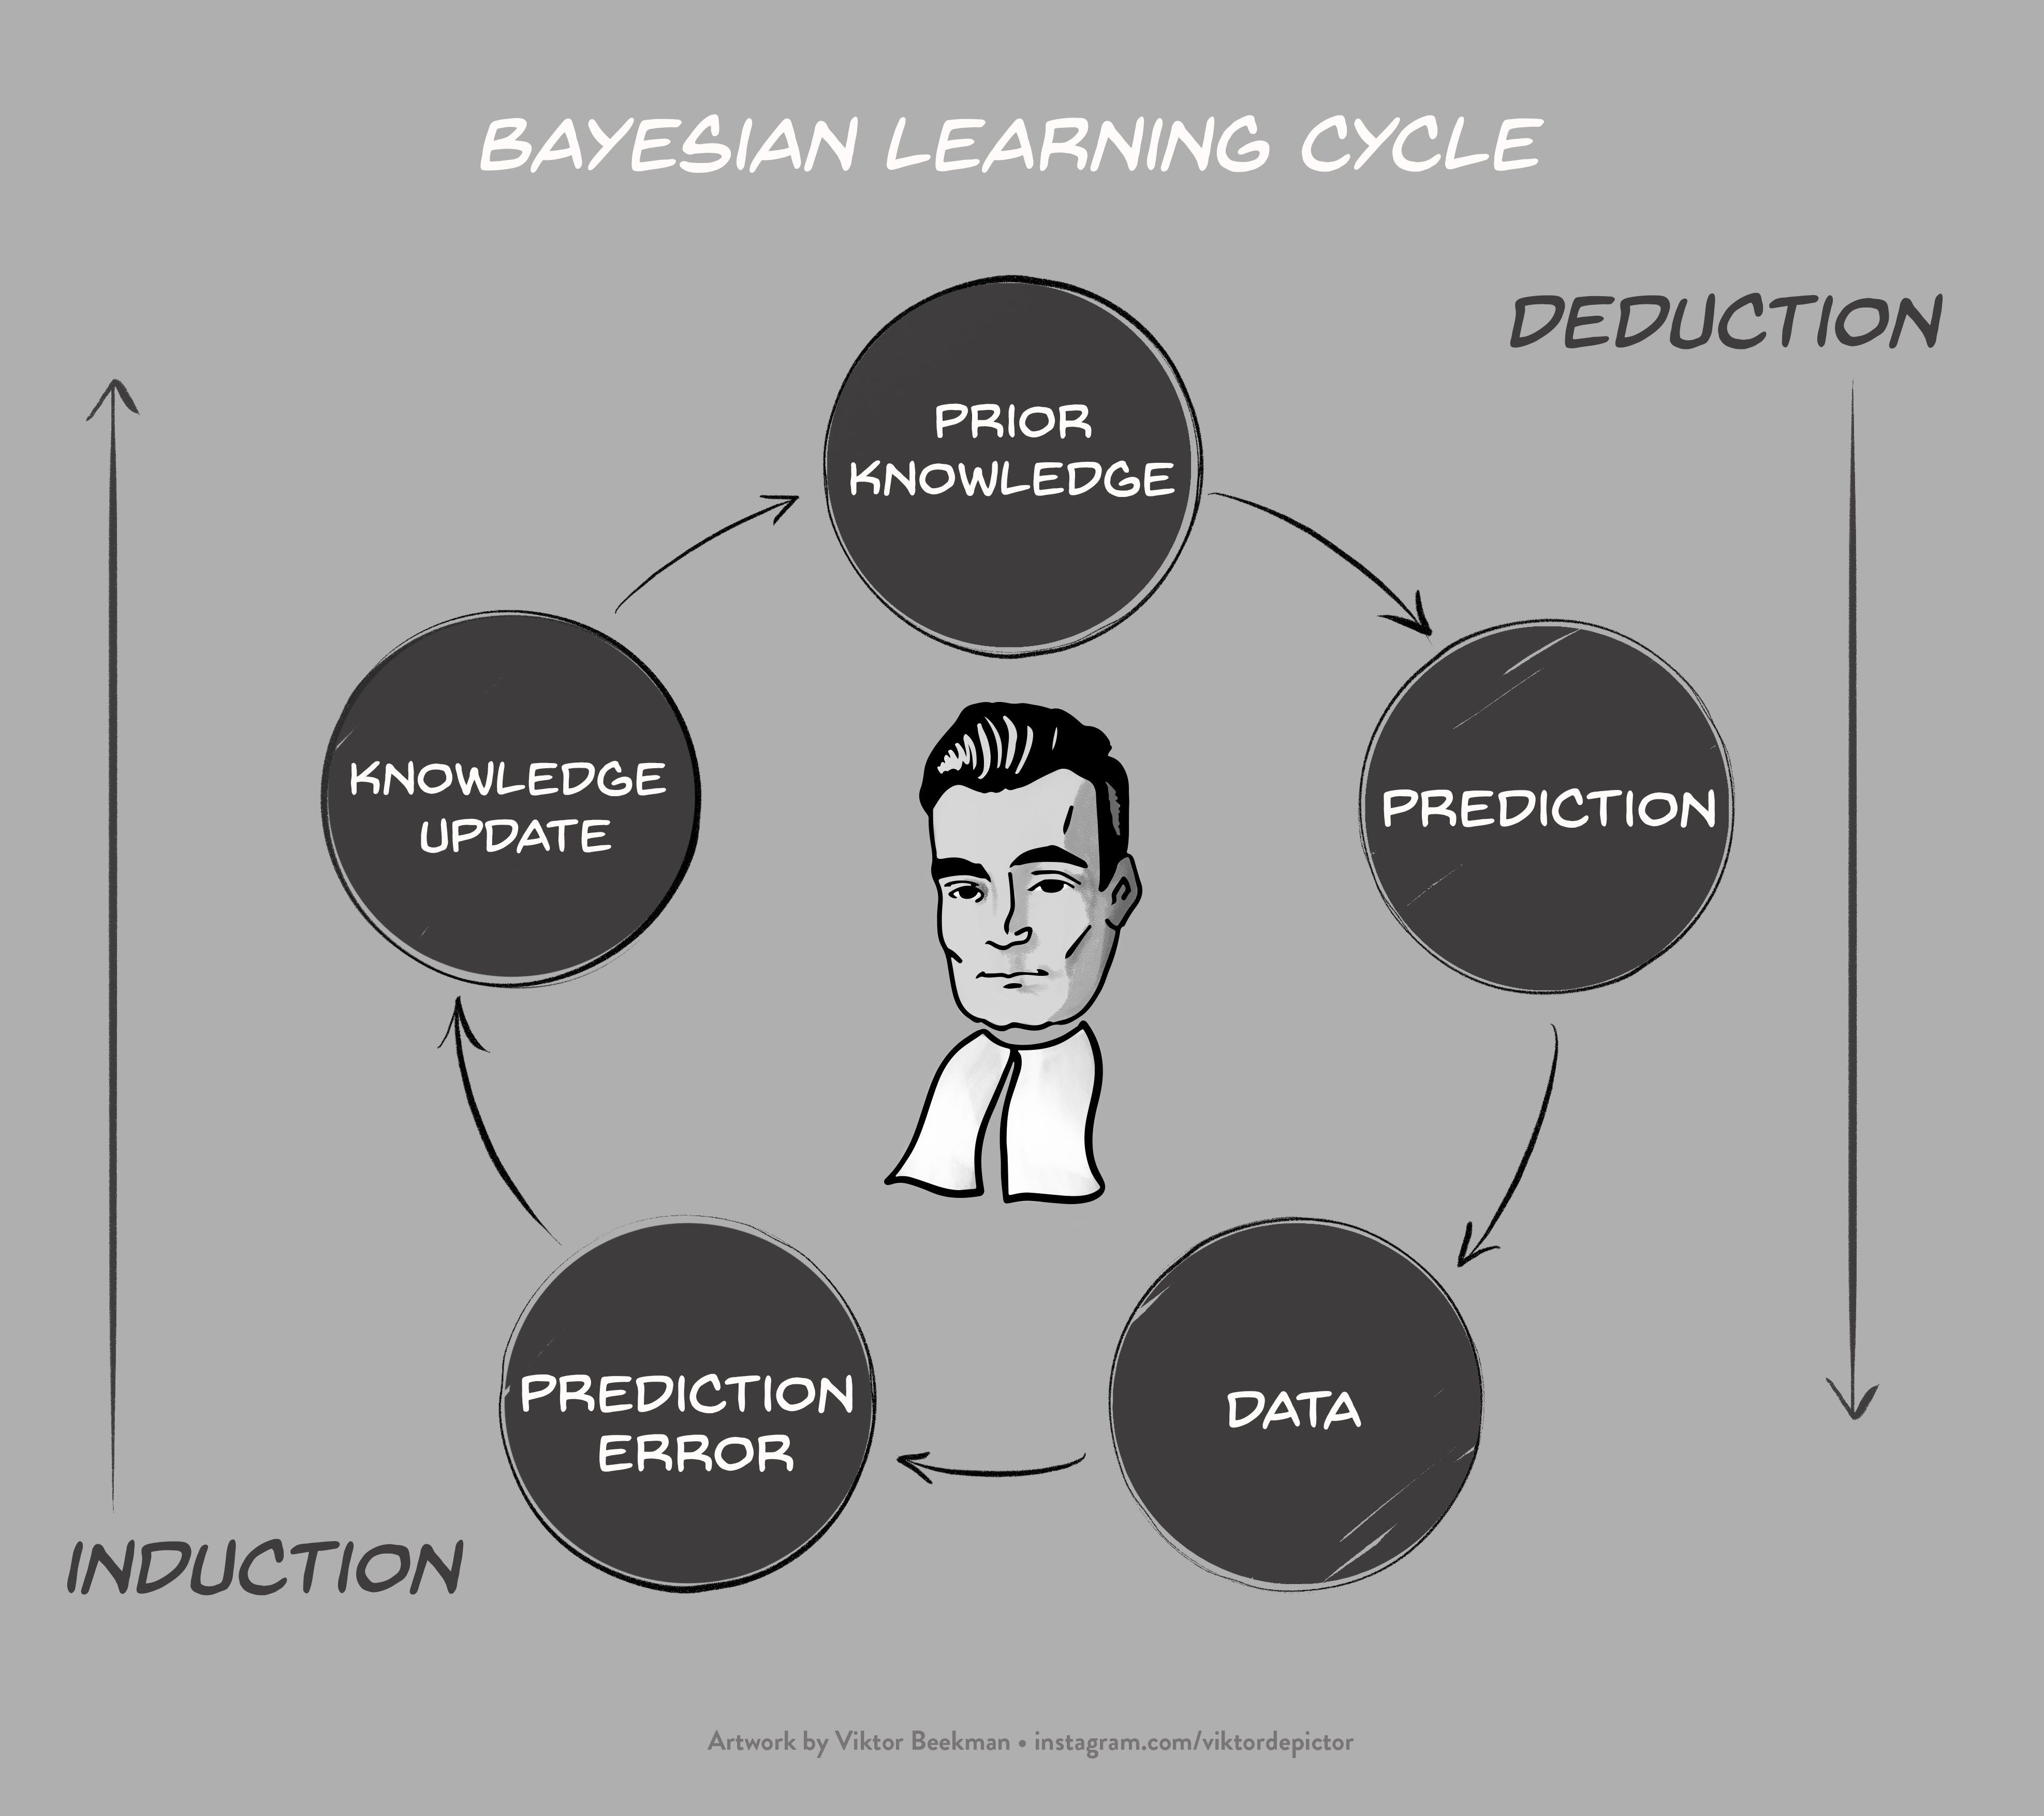
\includegraphics[width=1\linewidth]{Figures/BayesianLearningCycle} 

}

\caption{Bayesian learning cycle. }\label{fig:bayesian-learning-cycle}
\end{figure}

\hypertarget{the-lady-tasting-tea}{%
\chapter{The Lady Tasting Tea}\label{the-lady-tasting-tea}}

Over 80 years ago, Sir Ronald Fisher conducted the famous experiment ``The Lady Tasting Tea'' in order to test whether his colleague, Dr.~Muriel Bristol, could taste if the tea infusion or the milk had been added to the cup first \citep[p11]{fisher1937design}. Dr.~Bristol was presented with eight cups of tea and the knowledge that four of these had the milk poured in first. Dr.~Bristol was then asked to identify these four cups.
Fisher analyzed the results using null hypothesis significance testing:

\begin{enumerate}
\def\labelenumi{\arabic{enumi}.}
\tightlist
\item
  assume the null hypothesis to be true (i.e., Dr.~Bristol lacks any ability to discriminate the cups);
\item
  calculate the probability of encountering results at least as extreme as those observed;
\item
  if that probability is sufficiently low, consider the null hypothesis discredited.
\end{enumerate}

This probability is now known as the \(p\)-value and it features in many statistical analyses across empirical sciences.

\hypertarget{a-bayesian-version}{%
\section{A Bayesian Version}\label{a-bayesian-version}}

Decades later, Dennis \citet{Lindley1993} used an experimental procedure similar to that of Fisher to highlight some limitations of the \(p\)-value paradigm. Specifically, the calculation of the \(p\)-value depends on the sampling plan, that is, the \textit{intention} with which the data were collected. Consider the Lindley setup: Dr.~Bristol is offered six pairs of cups, where each pair consists of a cup where the tea was poured first, and a cup where the milk was poured first. She is then asked to judge, for each pair, which cup has had the tea added first. A possible outcome is the sequence RRRRRW, indicating that she was right for the first five pairs, and wrong for the last pair. However, as Lindley demonstrated, the original sampling plan is crucial in calculating the \(p\)-value because the \(p\)-value depends on hypothetical outcomes that are ``more extreme.''

Was the goal to have the Dr.~Bristol taste six pairs of cups --no more, no less-- or did she need to continue until she made her first mistake? The observed data could have been the outcome of either sampling plan; yet in the former case, the \(p\)-value equals \(0.109\), whereas in the latter case the \(p\)-value equals \(0.031\). The difference lies in the inclusion of more extreme cases. In the ``test six cups'' plan, the only more extreme outcome is RRRRRR (i.e., she correctly identified all 6 cups), whereas for the ``test until error'' plan the more extreme outcomes include sequences such as RRRRRRW and RRRRRRRW (i.e., 6 and 7 correct responses, before a single incorrect response)\footnote{A more technical way of describing the difference between the two setups is that data from the ``test six cups'' follow the binomial distribution, whereas data from the ``test until error'' follow the negative binomial distribution.}. It seems undesirable that the \(p\)-value depends on hypothetical outcomes that are in turn determined by the sampling plan. Harold Jeffreys summarized:
``What the use of \(p\) implies, therefore, is that a hypothesis that may be true may be rejected because it has not predicted observable results that have not occurred. This seems a remarkable procedure.'' \citep[p385]{Jeffreys1961}.

This drawback is one of the reasons (for more critique see \citep{Wasserstein2016, BenjaminEtAl2018}) why Bayesian inference has become more popular in the past years as an alternative framework for hypothesis testing and parameter estimation.

\hypertarget{an-alcoholic-version}{%
\section{An Alcoholic Version}\label{an-alcoholic-version}}

In this text we revisit Fisher's experimental paradigm to demonstrate several key concepts of Bayesian inference, specifically the prior distribution, the posterior distribution, the Bayes factor, and sequential analysis. Furthermore, we highlight the advantages of Bayesian inference, such as its straightforward interpretation, the ability to monitor the result in real-time, and the irrelevance of the sampling plan. For concreteness, we analyze the outcome of a tasting experiment that featured 57 staff members and students of the Psychology Department at the University of Amsterdam; these participants were asked to distinguish between the alcoholic and non-alcoholic version of the Weihenstephaner Hefeweissbier, a German wheat beer. We analyze and present the results in the open-source statistical software JASP \citep{JASP2022}.

\hypertarget{what-is-a-model}{%
\chapter{What is a Model?}\label{what-is-a-model}}

Before we dive into the analysis of the beer tasting experiment, we need to define some key components. First of all, the concept of a \emph{statistical model}. A statistical model is a combination of a general statistical model (e.g., the binomial model) and a statement about a parameter value that describe a certain phenomenon. For instance, we can model the flipping of a fair coin with the binomial model, where the probability parameter \(\theta\) (``theta'') is set to \(0.5\). Or, we can model the height of Dutch men (in cm) with a normal model, where the location parameter \(\mu = 183\) and the dispersion parameter \(\sigma = 5\). A statistical model can therefore also be seen as a hypothesis: a specific statement about the value of the model parameters.

\hypertarget{models-make-predictions}{%
\section{Models Make Predictions}\label{models-make-predictions}}

An essential property of a statistical model is that it can make predictions about the real world. We can use the accuracy of these predictions to gauge the quality/plausibility of a model, relative to another model. For instance,
Sarah thinks that the probability of heads in a coin flip is 50\% (i.e., \(H_S: \theta = 0.5\)), while Paul claims that the coin has been tampered with, and that the probability of heads is 80\% (i.e., \(H_P: \theta = 0.8\)). Here, Sarah and Paul postulate different models/hypotheses. They are both \href{https://en.wikipedia.org/wiki/Binomial_distribution}{binomial models}, which is the general statistical model for describing a series of chance-based events with a binary outcome (e.g., coin flip, red/black in roulette, whether a random person from the population has a certain disease or not, or someone identifying the alcholic beer). Where Sarah and Paul differ, however, is their claim about the specific value of the \(\theta\) parameter. In the remainder of this text, we will be refering to model to mean such a combination of general statistical model, and claim about the value of the model parameter (i.e., hypothesis).

\begin{figure}

{\centering 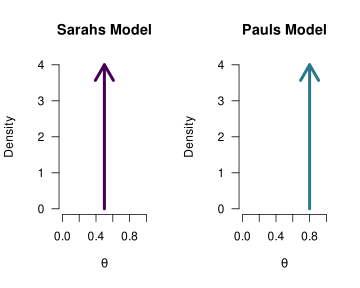
\includegraphics[width=0.9\linewidth]{_main_files/figure-latex/two-models-binomial-1} 

}

\caption{Two models for a coin toss. The arrows indicate what each of the models postulate: both postulate a single value for theta.}\label{fig:two-models-binomial}
\end{figure}

The two models make a different claim about \(\theta\), and therefore also make different \emph{predictions} about the outcome of a series of 10 coin flips. Specifically, we can use the binomial model to calculate how likely each possible outcome is under each of the models. For instance, we can calculate how likely it is to observe 8 heads out of 10 flips.
The binomial formula is as follows:
\begin{align} 
\label{binomFormula}
P(\text{data} \mid \theta) = \frac{n!}{k! (n-k)!} \theta^k\left(1-\theta\right)^{n-k},
\end{align}
which, if we fill in the outcome for which we want to know the likelihood (i.e., \(k=8\) heads out of \(n=10\) flips), becomes:
\[ P(\text{8 heads out of 10} \mid \theta) = \frac{10!}{8! (10-8)!} \theta^8\left(1-\theta\right)^{10-8}.\]
The last element to fill in is \(\theta\). If we do so for Sarah, who postulates \(\theta = 0.5\), we get 0.0439. For Paul, who postulates \(\theta = 0.8\), we get 0.302. If we do this for every possible outcome, and create a bar graph of each likelihood, we get the following two figures that illustrate what each model deems likely (the yellow bar indicates each models' likelihood of the example of 8 heads out of 10 flips):

\begin{figure}

{\centering 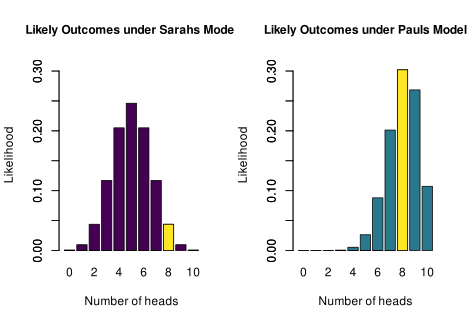
\includegraphics[width=0.9\linewidth]{_main_files/figure-latex/two-models-likelihoods-binomial-1} 

}

\caption{The likelihoods of all possible outcomes of 10 coin flips, under Sarahs model and under Pauls model. The yellow bar indicates the likelihood of the observed data (8 heads).}\label{fig:two-models-likelihoods-binomial}
\end{figure}

These two figures reflect likely outcomes of the experiment of flipping a coin 10 times. If Sarah is correct, and the probability of heads is in fact \(0.5\), likely outcomes are 4, 5, and 6. However, if Paul is correct, and \(\theta = 0.8\), it is more likely to see 7, 8 or 9 heads.

\hypertarget{model-comparison-section}{%
\section{Model Comparison}\label{model-comparison-section}}

In the previous section we have made concrete what each of the two models predict. The models differ in their statement about \(\theta\) (Figure \ref{fig:two-models-binomial}), and therefore differ in what they deem likely outcomes (Figure \ref{fig:two-models-likelihoods-binomial}). Now imagine that we actually gather some data by flipping a coin 10 times, and we observe 8 heads and 2 tails. Figure \ref{fig:two-models-likelihoods-binomial} tells us that the probability of that happening under Sarahs model is 0.0439, while under Pauls model this is 0.302. These two numbers tell us something about how well each model predicted the data, relative to each other. Specifically, the ratio of these two numbers is known as the \textbf{Bayes factor}. Here, the Bayes factor is equal to 0.15, which means that the observed data are about 0.15 times more likely under Sarahs model than under Pauls model.
The Bayes factor has a subscript that indicates what model is being compared to what: \(\text{BF}_{SP}\) gives how much more likely Sarahs model is than Pauls, while \(\text{BF}_{PS}\) gives how much more likely Pauls is than Sarahs. To go from \(\text{BF}_{SP}\) to \(\text{BF}_{PS}\), you simply take 1 divided by the other: \(\text{BF}_{PS}\) = \(\frac{1}{\text{BF}_{SP}}\) = 6.872. So saying that the data are 6.872 times more likely under Pauls model than Sarahs model is exactly the same. Generally, it is a bit easier to communicate the Bayes factor that is \(>1\), using the appropriate subscript.

Lastly, it can be the case that two models predicted the data equally well. In this case the Bayes factor will be equal to 1. Generally, we want the Bayes factor to be as far away from 1 as possible, since this indicates more and more evidence in favor of one model over another. Different categorizations have been made to translate a Bayes factor into human words, to facilitate communication about degrees of evidence for/against one model respective to another. One such representation is given below in Figure \ref{fig:bayes-factor-classification}.

\begin{figure}

{\centering 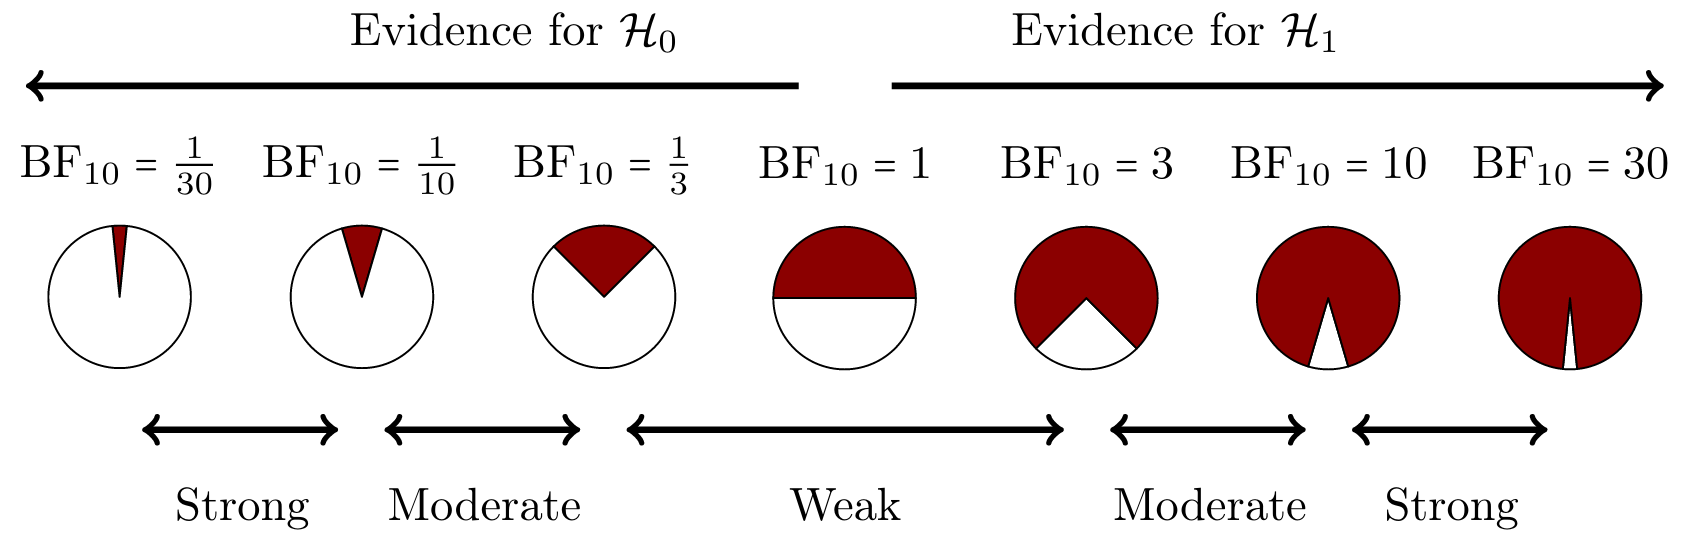
\includegraphics[width=0.9\linewidth]{Figures/BF_TableInterpretation} 

}

\caption{A graphical representation of a Bayes factor classification table. As the Bayes factor deviates from 1, which indicates equal support for $H_0$ and $H_1$, more support is gained for either $H_0$ or $H_1$. The probability wheels illustrate the continuous scale of evidence that Bayes factors represent. These classifications are heuristic and should not be misused as an absolute rule for binary all-or-nothing conclusions.}\label{fig:bayes-factor-classification}
\end{figure}

\hypertarget{more-models-section}{%
\section{More Models}\label{more-models-section}}

So far, we have considered two models (\(H_S\) and \(H_P\)), both of which postulate a single value for the model parameter \(\theta\). However, it is possible for a model to be more uncertain in its assertions. For instance, we can have a model that postulates that the probability of heads is greater than \(0.5\) (i.e., \(0.5 \leq \theta \leq 1\) \footnote{Because we are working with a continuous range of values for \(\theta\), the difference between saying \(0.5 < \theta\) and \(0.5 \leq \theta\) is infinitesimally small and the two versions may be used interchangeably.}). This corresponds to the belief that the coin is tampered with, but without making a strong statement about the degree of tampering. Furthermore, next to the model postulating the range for \(\theta\), it also needs to specify how likely it deems every value in this range. Let's add two more people and their models to the mix to illustrate. Betty believes the coin has been tampered with, but is unsure about the degree of tampering: she believes that every value of \(\theta\) between 0.5 and 1 is equally likely. Next is David, who is a bit more extreme in his beliefs: he believes that the coin is tampered with heavily, so assumes that values of \(\theta\) close to 1 are more likely than values of \(\theta\) closer to \(0.5\).
If we were to plot the models and corresponding hypotheses of Betty and David, they would look as follows (the difference in density reflecting their different beliefs):

\begin{figure}

{\centering 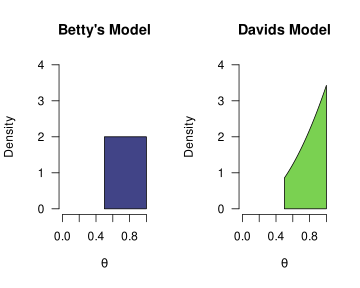
\includegraphics[width=0.9\linewidth]{_main_files/figure-latex/two-models-binomial-onesided-1} 

}

\caption{Two more models for a coin toss. The colored regions indicate what each model believes. Even though both Betty and David belive the probabilty of heads to be greater than 0.5, they differ in how plausible they deem specific values in that range.}\label{fig:two-models-binomial-onesided}
\end{figure}

Compared to the models in Figure \ref{fig:two-models-binomial}, which only ``bet'' on a single value, the models above spread their bets more. David and Betty thus make safer bets since they make wider predictions.
Although both Betty and David only consider positive values, they differ in how plausible they deem specific positive values. As before, these models also make predictions about how likely various outcomes of a series of 10 coin flips would be. Again, the binomial formula can be used. However, this time the models do not predict a single value, but a whole range of values. In order to compute how likely Betty's model deems an outcome of 8 heads out of 10 flips, we have to consider every postulated value of \(\theta\) between 0.5 and 1, compute the likelihood of the data for each value, and average across all of these likelihoods, weighted by the density at each point. The technical term for such weighted averaging is called marginalizing, and we refer to this averaged likelihood as the \textbf{marginal likelihood}. In the next section we will revisit this topic.

In Figure \ref{fig:two-models-binomial-onesided-predictions} below, you can see the marginal likelihoods for all outcomes, for each of the two additional models. Note that even though neither Betty nor David postulate values of \(\theta\) below 0.5 (i.e., the \emph{parameter}), they assign some plausibility to observed proportions below 0.5 (i.e., the \emph{statistic}, or observed data). This reflects the random nature of a coin flip: even though the true probability of heads is \(0.6\), you might still observe 3 heads out of 10 flips.

\begin{figure}

{\centering 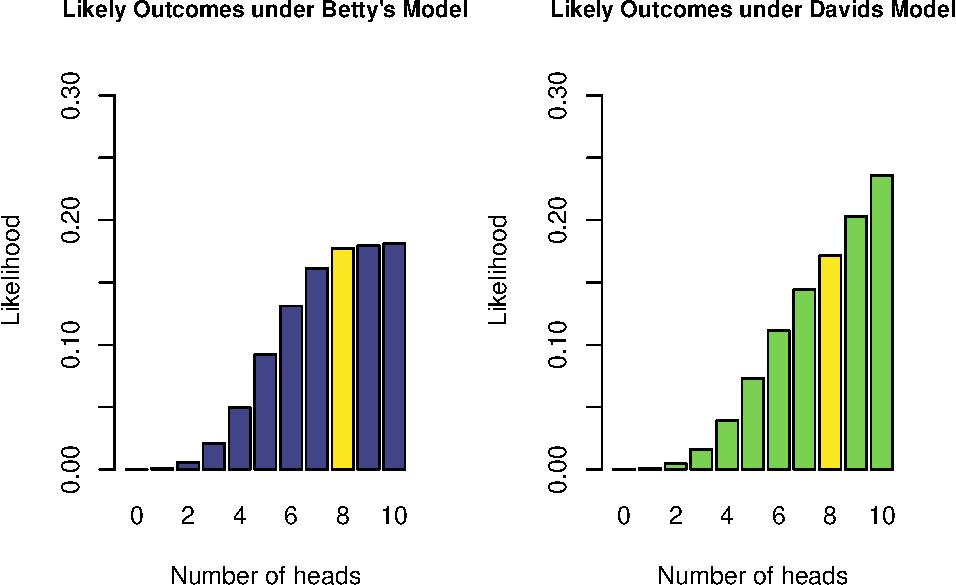
\includegraphics[width=0.9\linewidth]{_main_files/figure-latex/two-models-binomial-onesided-predictions-1} 

}

\caption{The marginal likelihoods of all possible outcomes of 10 coin flips, under the two additional models. The yellow bar indicates the marginal likelihood of the observed data (8 heads).}\label{fig:two-models-binomial-onesided-predictions}
\end{figure}

\hypertarget{open-minded-model-section}{%
\subsection{The Open-Minded Model}\label{open-minded-model-section}}

Lastly, but perhaps most importantly, we can also consider a model that tries to spread its bets as much as possible. Let's say that Alex wants to keep as much of an open mind about values of \(\theta\) as possible. They consider each possible value of \(\theta\) to be equally plausible. In Bayesian inference, we also refer to this type of model as the \emph{uninformed} model. The figure below illustrates what the uninformed model posits, and which outcomes it deems likely. We again have a model that postulates multiple values, so the figure on the right depicts marginal likelihoods. For instance, for the yellow bar, we look at how likely 8 heads out of 10 flips are, averaged over all values postulated by the model, weighted by the density in the left graph.

\begin{figure}

{\centering 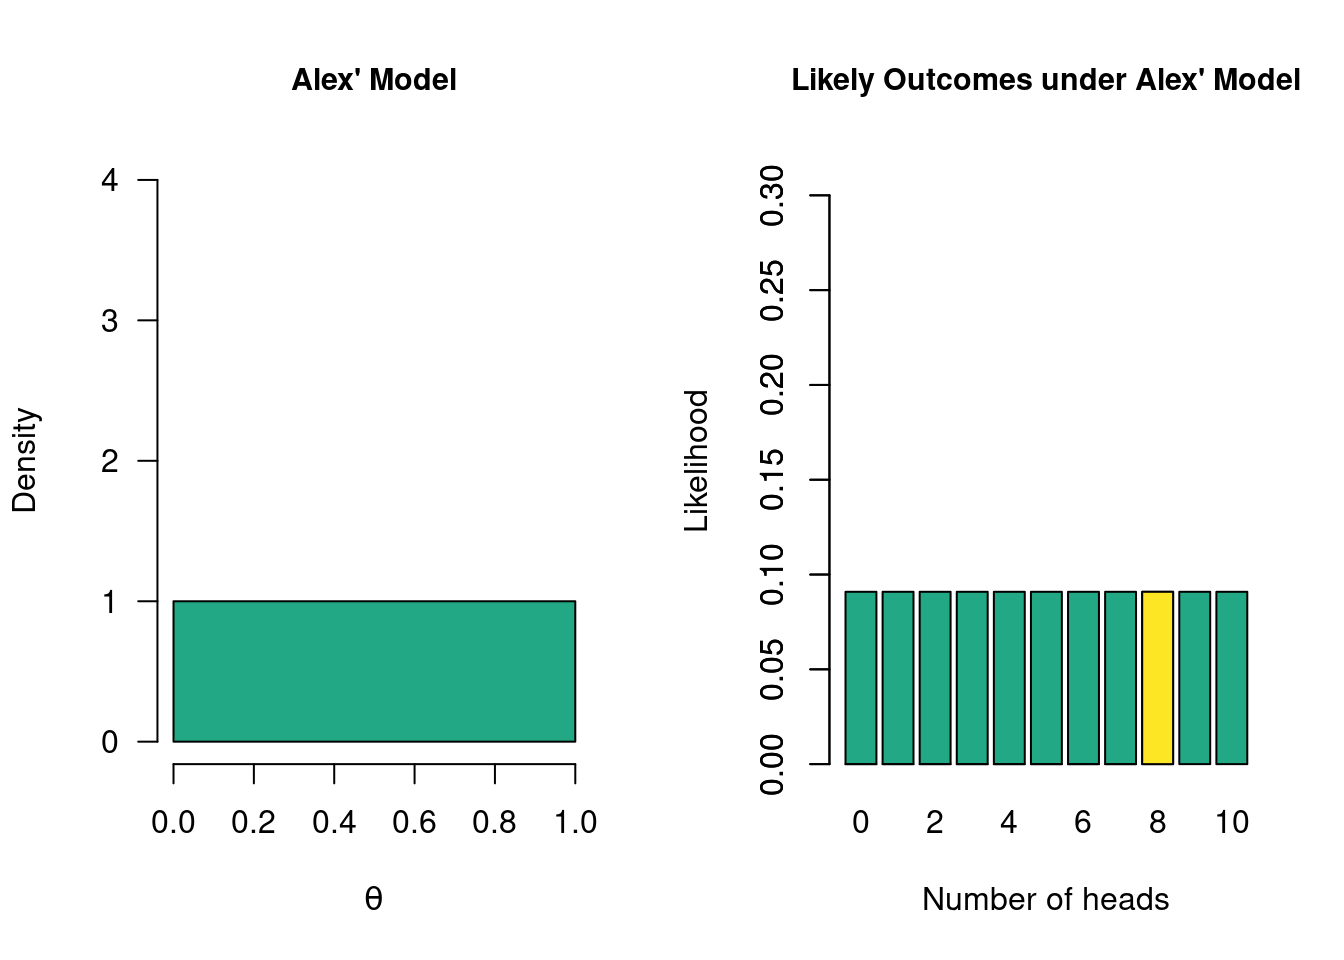
\includegraphics[width=0.9\linewidth]{_main_files/figure-latex/uninformed-model-binomial-prediction-1} 

}

\caption{The so-called "uninformed model". Alex wants to keep an open mind about the values of theta and considers each value equally plausible. Left: the colored region indicate what Alex believes. Right: what this specific model considers likely outcomes. The yellow bar indicates the marginal likelihood of the observed data (8 heads).}\label{fig:uninformed-model-binomial-prediction}
\end{figure}

\hypertarget{more-model-comparison-section}{%
\section{More Model Comparisons}\label{more-model-comparison-section}}

We can apply the same principles from section \ref{model-comparison-section} to compare how well each of the additional models has predicted the observed data of 8 heads out of 10 coin flips. To do so, we can simply take the ratio of each of the yellow bars in the figures that depict how likely each model considers the various possible outcomes of 10 coin flips. For instance, Alex' model has a marginal likelihood of 0.0909 for 8 heads, whereas Betty's model has a marginal likelihood of 0.1754 for 8 heads. If we want to compare the predictions of Betty and Alex, we can look at the ratio of these values to obtain \(\text{BF}_{AB} =\) 0.5, which is equivalent to \(\text{BF}_{BA} =\) 1.9. This means that the data are about twice as likely under Betty's model than under Alex' model, which can be considered weak evidence in favor of Betty's model over Alex' model.

If we were to use the betting analogy again, we could say that while both Alex and Betty had bet some money on the outcome of 8 heads, Betty had bet more money on this particular outcome than Alex, and is therefore rewarded more. Because Betty has a more specific belief (namely that the coin is biased towards heads), she had more money at her disposal for betting on the considered values (i.e., values between 0.5 and 1). In contrast, Alex played it very safely: they win some money for any outcome because they spread their betting money across all values. However, because of this, their reward is lower for having correctly predicted the observed data compared to someone who made a more specific bet on the observed data. The phenomenon of more specific models being rewarded more (when predicting well) than their non-specific competitor is known as \textbf{parsimony}, and will be discussed in more depth in Chapter 4.

A last model comparison we can make is to compare Alex' model to Sarah's model. In a typical (two-sided) statistical test about a proportion, this is the most often-used comparison: Sarah's model is considered to be the null model, and Alex' model is considered the two-sided alternative model. As we saw, Alex' marginal likelihood is 0.0909, while Sarah's marginal likelihood is 0.0439, so the Bayes factor comparing these two models, \(\text{BF}_{AS}\), equals 2.07. This means the data are about twice as likely under Alex' model compared to Sarah's model.

As a bonus, when we know \(\text{BF}_{BA}\) and \(\text{BF}_{AS}\), we automatically know \(\text{BF}_{BS}\). Since we know how many more times Betty's model is than Alex' (about 2 times), and how many more times Alex' model is than Sarah's (about 2 times), we also now know that Betty's model is about \(2 \times 2 = 4\) times more likely than Sarah's model! This property it known as \textbf{transitivity}.

\hypertarget{concluding-thoughts}{%
\section{Concluding Thoughts}\label{concluding-thoughts}}

In this chapter, we have seen several key ideas:

\begin{itemize}
\tightlist
\item
  Models make concrete statements about parameters of a model. In this case, about the \(\theta\) parameter in the binomial model
\item
  These statements can be characterized by a probability distribution, where the probability mass reflects the specific statement

  \begin{itemize}
  \tightlist
  \item
    The model could hypothesize a single value (e.g., \protect\hyperlink{fig:two-models-binomial}{the models of Sarah and Paul})
  \item
    The model could hypothesize a range of values (e.g., \protect\hyperlink{fig:two-models-binomial-onesided}{the models of Betty, David} and \protect\hyperlink{fig:uninformed-model-binomial-prediction}{Alex})
  \end{itemize}
\item
  After we have observed some data, we can use the Bayes factor to compare the quality of the predictions made by each model

  \begin{itemize}
  \tightlist
  \item
    The Bayes factor is a relative metric, comparing 2 models at a time
  \item
    The subscript of the Bayes factor indicates which model is compared to which
  \item
    More specific predictions, when accurate, are rewarded (parsimony)
  \end{itemize}
\end{itemize}

Instead of comparing models, however, we can also look at one model, and use it to \textbf{estimate} the value of \(\theta\). We will see that each of the models presented above will yield different estimates, because they had different \emph{a priori} (i.e., before seeing the data) beliefs about plausible values of \(\theta\).

\hypertarget{model-estimation-section}{%
\chapter{How do Models Estimate?}\label{model-estimation-section}}

In the previous chapter, we saw that people/models can have different beliefs/hypotheses about a phenomenon. Sarah was quite certain that the true probability of the coin landing heads was \(0.5\), whereas David believed that the coin was biased towards heads, assigning more mass to higher values of \(\theta\). We saw how we can observe data to test which of the models predicted this data the best, using the Bayes factor. In this chapter, we will look at how individual models update their beliefs, as a result of observing the data. In doing so, this chapter will illustrate the core Bayesian concept of starting with \textbf{prior} knowledge/beliefs, updating this knowledge with observed data, to end up with \textbf{posterior} knowledge/beliefs about a parameter.

The following formula reflects this process:
\begin{align}
\label{eq:BinomialEstimation}
\underbrace{ p(\theta \mid \text{data})}_{\substack{\text{Posterior beliefs}}} \,\,\, = \,\,\,
\underbrace{ p(\theta)}_{\substack{\text{Prior beliefs} }}
\,\,\,\, \times
\overbrace{\underbrace{\frac{p( \text{data} \mid \theta)}{p( \text{data})}}}^{\substack{\text{Prediction for specific }\theta }}_{\substack{\text{Average prediction} \\\text{across all }  \theta's}}.
\end{align}
We have prior beliefs, which are updated by an \textbf{updating factor}, to form posterior beliefs. The updating factor indicates for each possible value of \(\theta\), how well it predicted the observed data, relative to all other possible values of \(\theta\). If this is still sounding rather vague, don't worry - in this section we will demonstrate how this updating factor operates. However, before we discuss the updating factor, we go back to the start, and discuss the concept of prior knowledge/beliefs.

\hypertarget{models-have-beliefs}{%
\section{Models Have Beliefs}\label{models-have-beliefs}}

Belief is a funny word and we tend to associate the word with things that have seemingly little to do with science or statistics. However, we have beliefs about anything in the world -- they might be quite weak, but we still have \emph{some} starting point for reasoning about some phenomenon. For instance, I know very little about the number of penguins in the world, but I do know there are more than 0, probably more than \(1{,}000\), and fewer than \(1{,}000{,}000{,}000\) of them.\footnote{How would you characterize your beliefs about the number of penguins in the world? What would your belief distribution look like?} I could characterize my very uninformed belief by means of a proability distribution, where the probabilty mass depicts how plausible I deem certain values. This is exactly the same as we did in the previous chapter by characterizing the different peoples' beliefs about the fairness of a coin. In this case, even if we would know absolutely nothing about the coin in question, we still have \emph{some} information about the parameter \(\theta\). For instance, we know that it will be between 0 and 1 because it is a probability. If we do not have any knowledge beyond this, we could reflect our prior belief about \(\theta\) by means of a uniform distribution, just like Alex did. In fact, we will now illustrate belief updating by looking at how Alex updates their beliefs, as a result of observing 8 heads out of 10 flips.

\hypertarget{updating-beliefs}{%
\section{Updating Beliefs}\label{updating-beliefs}}

As you might recall from section \ref{open-minded-model-section}, Alex was keeping an open mind about the values \(\theta\) - their \textbf{prior distribution}\footnote{The prior distribution is the offical term for the probability distribution that quantifies a model's prior beliefs about a parameter.} was a uniform distribution across all values between 0 and 1.

\begin{figure}

{\centering 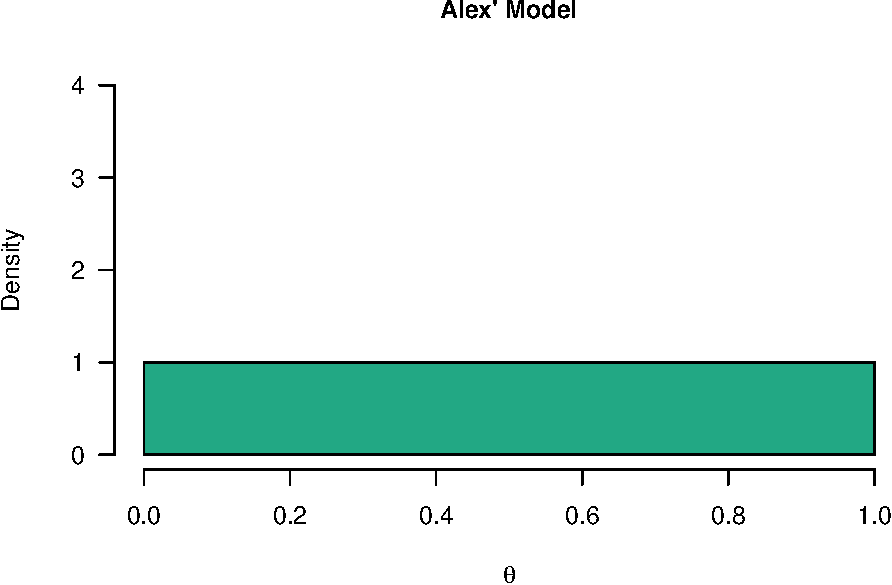
\includegraphics[width=0.9\linewidth]{_main_files/figure-latex/uninformed-model-binomial-prediction-2-1} 

}

\caption{The so-called "uninformed model". Alex wants to keep an open mind about the values of theta and considers each value equally plausible. The uniform prior distribution below reflects this.}\label{fig:uninformed-model-binomial-prediction-2}
\end{figure}

Now that we have formalized the prior beliefs about a parameter in the form of a probability distribution, we can start updating those beliefs with observed data. The belief updating factor consists of two parts.

\hypertarget{the-likelihood}{%
\subsection{The Likelihood}\label{the-likelihood}}

The first part of the updating factor, \(p( \text{data} \mid \theta)\), expresses the likelihood of the observed data for all of the values postulated by the model. Here, this means all values between 0 and 1. For instance, we look at the likelihood of the observed data, given a \(\theta\) value of 0.1. Just as before, we can use the binomial formula for this:
\begin{align} 
\label{binomFormulaTwo}
\frac{n!}{k! (n-k)!} \theta^k\left(1-\theta\right)^{n-k},
\end{align}
which for \(n = 10\), \(k = 8\), and \(\theta = 0.1\) gives 0. We can compute this value for all of the values between 0 and 1. If we do so, we can make the following graph that shows the likelihood of the data, for each value of \(\theta\):

\begin{figure}

{\centering 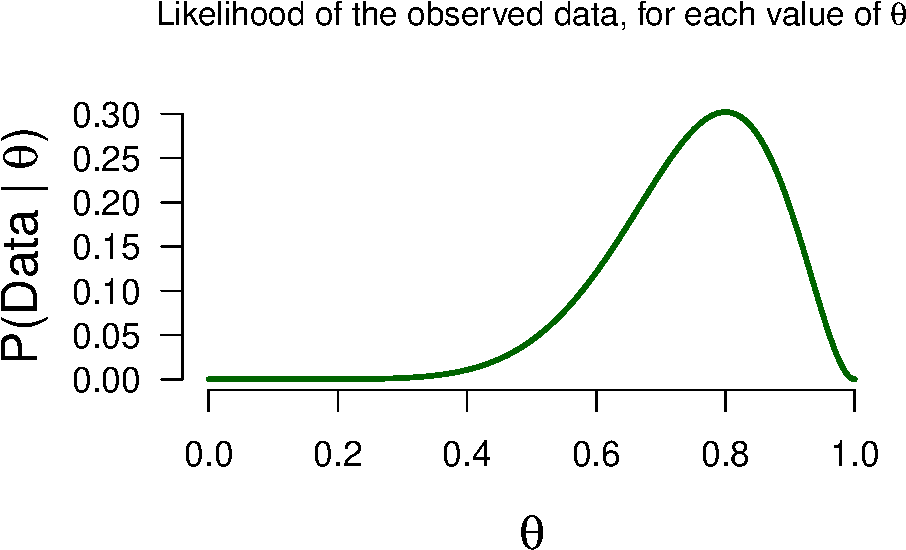
\includegraphics[width=0.9\linewidth]{_main_files/figure-latex/likelihood-binomial-8-heads-1} 

}

\caption{The likelihood of observing 8 heads out of 10 flips, for all possible values of theta.}\label{fig:likelihood-binomial-8-heads}
\end{figure}

As you can see, the likelihood is the greatest for \(\theta = 0.8\). This makes sense because the observed proportion is equal to \(0.8\). In short, this likelihood function depicts how well each possible value of \(\theta\) predicted the observed data. In the previous section we saw two people who postulated only a single value for \(\theta\). The likelihoods of their models can also be read from the above graph: Sarah (\(P(\text{data} \mid \theta = 0.5) =\) 0.0439) and Paul (\(P(\text{data} \mid \theta = 0.8) =\) 0.302).

It is important to note that the likelihood is \textbf{not} a probability distribution: its surface area does not sum to 1, and we therefore cannot use it to make probabilistic statements about the parameter (we can use the posterior distribution for this, at the end of this section).

\hypertarget{the-marginal-likelihood}{%
\subsection{The Marginal Likelihood}\label{the-marginal-likelihood}}

Now we can take a look at the second part of the updating factor: \(p( \text{data})\). This part is known as the \textbf{marginal likelihood}. In contrast to the first part, the marginal likelihood is a single number. Namely, it is the average of all the likelihoods, where the likelihood of each value is weighted by the prior belief placed on that value by the model. This is the same procedure as in the previous chapter (see section \ref{more-models-section}). In fact, for all of the models, the marginal likelihood was indicated by the yellow bar: it is the likelihood of the observed data, weighted by each model's specific beliefs.
In the case of Alex' model, the prior belief is equal across all values, so the marginal likelihood is ``simply'' the average likelihood.\footnote{Technical sidenote: \emph{integrating} over the likelihood will give the marginal likelihood for Alex.} In this case, the marginal likelihood is equal to 0.0909 - precisely the height of the yellow bar in Figure \ref{fig:uninformed-model-binomial-prediction}.

We can use this average likelihood to see which possible values of \(\theta\) predicted the data better than average, and which values predicted the data worse than average: since the likelihood reflects the predictive quality of each value, the marginal likelihood reflects the average quality across all values.
In the following figure, you can again see the likelihood function from Figure \ref{fig:likelihood-binomial-8-heads}, but now with the marginal likelihood added:

\begin{figure}

{\centering 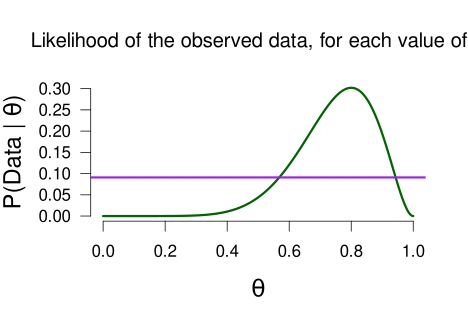
\includegraphics[width=0.9\linewidth]{_main_files/figure-latex/likelihood-binomial-8-heads-marginal-1} 

}

\caption{The likelihood of observing 8 heads out of 10 flips, for all possible values of theta. The purple line is the marginal likelihood, to visualize which values predicted the observed data better than average.}\label{fig:likelihood-binomial-8-heads-marginal}
\end{figure}

By doing so, we have quite literally set the bar: values of \(\theta\) where the likelihood is greater than the marginal likelihood (approximately values between \(0.55\) and \(0.95\)) predicted the data better than average. In other words, \(p( \text{data} \mid \theta) > p( \text{data})\). This means that the updating factor (i.e., the ratio of the likelihood and marginal likelihood) will be greater than 1. This in turn means that the posterior belief for those values will be greater than the prior belief. As a result of observing the data, values between \(0.55\) and \(0.95\) have an increase in plausibility. The reverse holds for values whose likelihood is lower than the marginal likelihood: those values have suffered a decrease in plausibility as a result of the data.
Perhaps another look at the Bayesian updating formula makes more sense now than it did at first:
\begin{align}
\underbrace{ p(\theta \mid \text{data})}_{\substack{\text{Posterior beliefs}}} \,\,\, = \,\,\,
\underbrace{ p(\theta)}_{\substack{\text{Prior beliefs} }}
\,\,\,\, \times
\overbrace{\underbrace{\frac{p( \text{data} \mid \theta)}{p( \text{data})}}}^{\substack{\text{Prediction for specific }\theta }}_{\substack{\text{Average prediction} \\\text{across all }  \theta's}}.
\end{align}

We can visualize the aforementioned process. Again we look at the likelihood values, but now the values that see an increase/decrease in plausibilty are marked by the blue/vermillion arrows, respectively:

\begin{figure}

{\centering 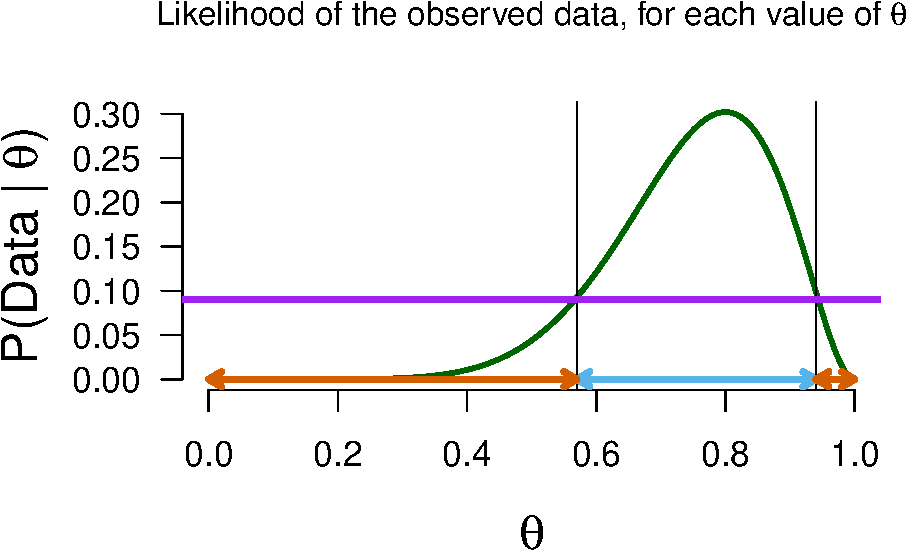
\includegraphics[width=0.9\linewidth]{_main_files/figure-latex/likelihood-binomial-8-heads-marginal-redgreen-1} 

}

\caption{Values of theta that predicted the data better than average (marked in blue) will have a updating factor greater than 1, and receive a boost in plausibility as a result of the data. The reverse holds for values that predicted worse than average (marked in vermillion). }\label{fig:likelihood-binomial-8-heads-marginal-redgreen}
\end{figure}

\hypertarget{updated-beliefs}{%
\section{Updated Beliefs}\label{updated-beliefs}}

We started this section with the prior beliefs of Alex' model, which we updated by looking at which values predicted the data well, in order to form posterior beliefs. Just as with prior beliefs, our posterior beliefs are in the form of a posterior distribution. The figure below shows both distributions, including the vertical lines from Figure \ref{fig:likelihood-binomial-8-heads-marginal-redgreen} to illustrate the boost/penalty in plausibility.

\begin{figure}

{\centering 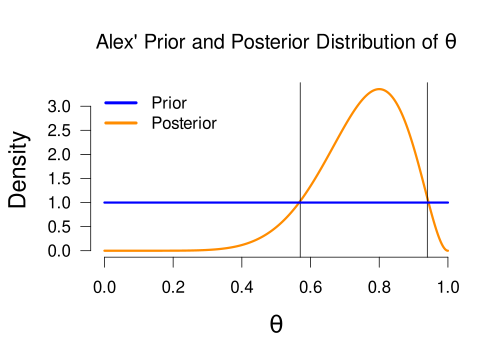
\includegraphics[width=0.9\linewidth]{_main_files/figure-latex/prior-posterior-binomial-1} 

}

\caption{Prior and posterior distribution. }\label{fig:prior-posterior-binomial}
\end{figure}

We have now updated Alex' prior knowledge to posterior knowledge! The posterior distribution enables us to make probabilistic statements about values of \(\theta\) because it is a probability distribution.\footnote{Note the contrast to the sampling distribution, which is a distribution of the sample statistic \(\hat{p}\), rather than the parameter.} For instance, the median of this posterior distribution is \(0.764\), which means that under Alex' model, there is a 50\% probability that \(\theta\) is greater than \(0.764\). Or, we can use the posterior distribution to make an \emph{interval estimation}. In the Bayesian framework, this is known as the \textbf{credible interval}. This interval entails taking the middle \(x\)\% of the posterior distribution. For instance, we can take a 95\% credible interval, which ranges from \(0.482\) to \(0.940\) in this case. This means that under Alex' model, there is a 95\% probability that the true value of \(\theta\) is between \(0.482\) and \(0.940\). Such a straightfoward interpretation is one of the strengths of the Bayesian framework, compared to the frequentist framework.

\hypertarget{more-models}{%
\section{More Models}\label{more-models}}

Up until this point, we have only looked at Alex' model: it had a specific starting point (i.e., prior belief), which was updated with the observed data to form an ending point. However, in the previous chapter we saw that there are all sorts of different models. Each of those models have different prior beliefs (as reflected by their prior distributions). Even though the Bayesian knowledge updating procedure is exactly the same for all models, having a different starting point means that they also have a different ending point. Specifically, for each model, their prior distribution is different, and their marginal likelihood is different (as indicated by the yellow bars in the Figures in the previous chapter).

The models shown so far differ in their ``learning ability''. Generally, the uninformed model is a great learner: because it has a relatively weak starting point, it lets the data speak for itself. This is reflected by the posterior distribution being highly similar to the likelihood.\footnote{Remember that the likelihood is not a probability distribution. You can see Bayesian statistics as a ``trick'' to turn the likelihood into a probability distribution (i.e., the posterior distribution), so that you can make probabilistic statements about the parameter!} In order to illustrate the differences in the models, and how they learn, we can go over how Sarah's model and David's model learned from the data.

\hypertarget{sarahs-learning-process}{%
\subsection{Sarah's Learning Process}\label{sarahs-learning-process}}

While Alex was casting a very wide net, Sarah was doing the opposite. Rather than considering all values of \(\theta\), Sarah was absolutely sure that there was only one possible value of \(\theta\), namely \(0.5\).

\begin{figure}

{\centering 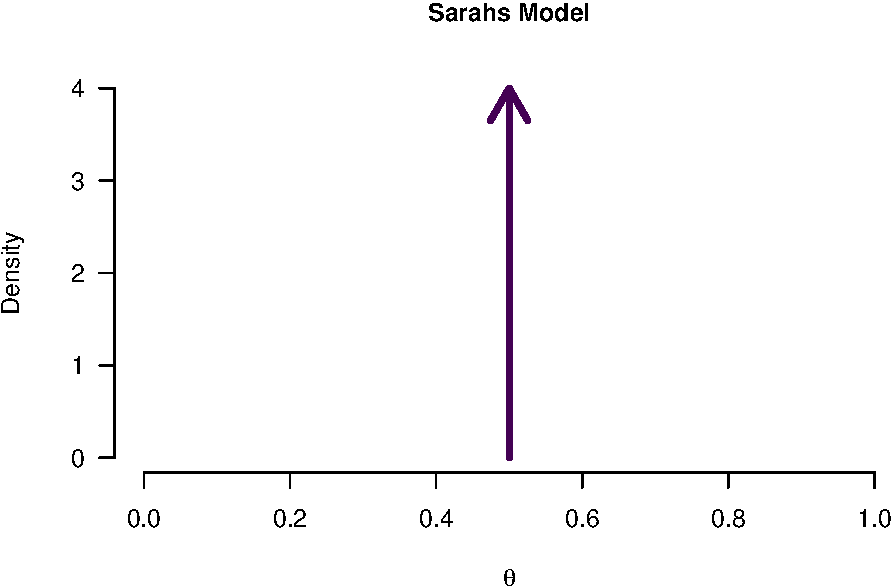
\includegraphics[width=0.9\linewidth]{_main_files/figure-latex/sarah-model-binomial-1} 

}

\caption{Sarah's model for a coin toss. The arrow indicates that only a single value for theta is postulated.}\label{fig:sarah-model-binomial}
\end{figure}

In other words, Sarah's prior belief about \(\theta\) was quite fanatical. The prior density of all values other than 0.5 is 0, and the prior density at 0.5 is infinitely high (since infinity cannot be conveniently shown in a figure, we use the arrow to indicate infinity). So what happens when someone is absolutely convinced that \(\theta = 0.5\), and then gets presented with data? Perhaps another look at the Bayesian updating formula can give some insight:
\begin{align}
\underbrace{ p(\theta \mid \text{data})}_{\substack{\text{Posterior beliefs}}} \,\,\, = \,\,\,
\underbrace{ p(\theta)}_{\substack{\text{Prior beliefs} }}
\,\,\,\, \times
\overbrace{\underbrace{\frac{p( \text{data} \mid \theta)}{p( \text{data})}}}^{\substack{\text{Prediction for specific }\theta }}_{\substack{\text{Average prediction} \\\text{across all }  \theta's}}.
\end{align}

Since Sarah's prior density for any value that is not 0.5, is equal to 0, that means that the posterior density for those values will also be 0. Because of the multiplication by 0, the updating factor is therefore completely ignored. As for the pior density at the value 0.5 - it too gets mutliplied by the updating factor, but just as anything multiplied by 0 is 0, anything multiplied by infinity is infinity. In other words, a model like Sarah's is completely blind to the data, since she is alread so convinced that \(\theta = 0.5\).\footnote{I feel like there is a real-life analogue to be found here somewhere\ldots{}} The posterior will therefore be exactly the same as in Figure \ref{fig:sarah-model-binomial} above.

Let's define the marginal likelihood once more: Sarah has prior beliefs about \(\theta\), reflected by the prior mass in Figure \ref{fig:sarah-model-binomial}. Each of these values has a certain match with the observed data (i.e., the likelihood). The marginal likelihood is then the average of all those likelihoods, weighted by the prior mass assigned. This weighting by prior mass makes each model's marginal likelihood different from each other, because each has their own unique prior beliefs.
If we were to look at the updating factor for Sarah, we would see that Sarah's marginal likelihood is simply equal to the likelihood of the data for \(\theta = 0.5\) (i.e, \(P(\text{data} \mid \theta = 0.5) =\) 0.0439) because that is the only value that Sarah assigned any prior mass to.

\hypertarget{davids-learning-process}{%
\subsection{David's Learning Process}\label{davids-learning-process}}

Somewhere in the middle of Alex' ambivalence and Sarah's fanaticism, there is David's prior belief that only values between 0.5 and 1 are possible, and that values closer to 1 are more plausible than values closer to 0.5. As you can see in Figure \ref{fig:david-model-binomial} below, this means that values between 0 and 0.5 are assigned 0 prior density - a process known as \textbf{truncation}. Truncation makes a model \textbf{one-sided}, since only values to one side of 0.5 have been assigned prior density, while the other side is set to 0. From Sarah's learning process we saw that this means that David's \emph{posterior} beliefs will also be 0 for values below 0.5. So what does David's learning process look like?

\begin{figure}

{\centering 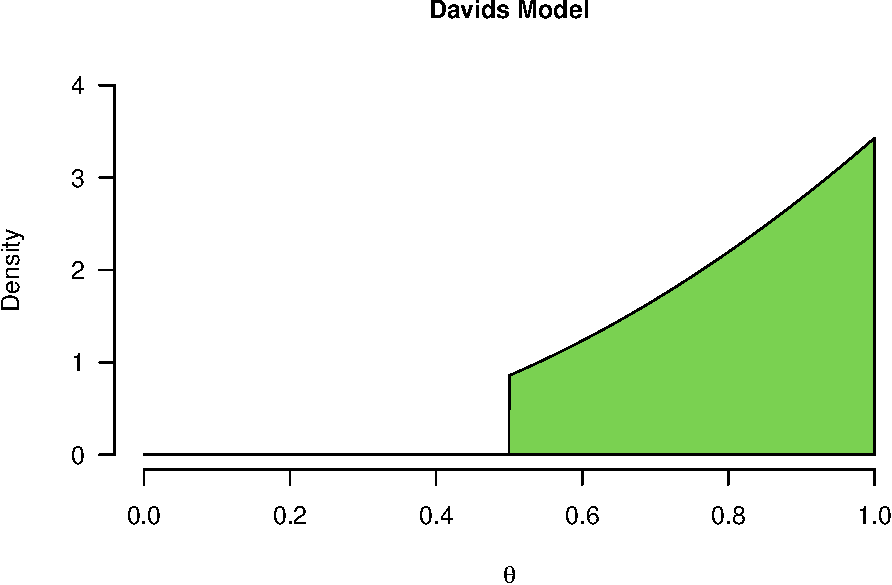
\includegraphics[width=0.9\linewidth]{_main_files/figure-latex/david-model-binomial-1} 

}

\caption{David's model for a coin toss. David believes that only values between 0.5 and 1 are possible, and that values closer to 1 are more plausible, a priori. When certain ranges of values have their density set to 0, we refer to the distribution as a *truncated distribution*.}\label{fig:david-model-binomial}
\end{figure}

Just as before, we start with the prior beliefs, update these with the updating factor (which values in the model predicted the data better/worse than average?), to form posterior beliefs. The difference between the different models lies in their different starting points (prior beliefs), but also their updating factor differs. Specifically, the likelihood stays the same (Figure \ref{fig:likelihood-binomial-8-heads}), but the marginal likelihood differs. As we see in Figure \ref{fig:two-models-binomial-onesided-predictions}, David's marginal likelihood for the outcome of 8 heads is approximately 0.175.

In the previous chapter we saw how we can use the ratio of the marginal likelihoods of two models (i.e., the Bayes factor) to do model comparison. In this chapter we focus on individual models and how they estimate/learn about the parameter. In that context we use the marginal likelihood to see which parameter values in the model predicted the data better/worse than average, in order to see which values receive a boost/penalty in plausibility. The figure below illustrates this mechanism - note that the likelihood is exactly the same as for other models, but the marginal likelihood (indicated by the purple bar) is different.

\begin{figure}

{\centering 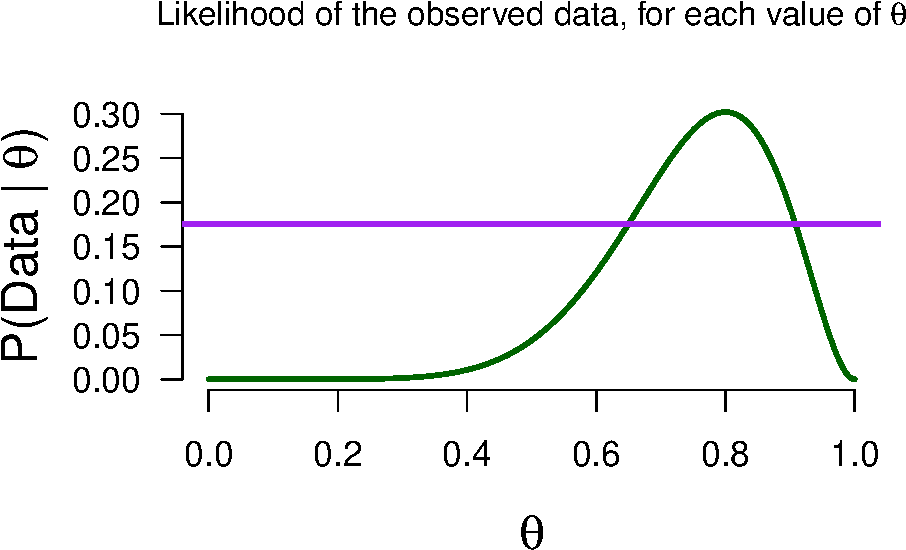
\includegraphics[width=0.9\linewidth]{_main_files/figure-latex/likelihood-binomial-8-heads-marginal-david-1} 

}

\caption{The likelihood of observing 8 heads out of 10 flips, for all possible values of theta. The purple line is the marginal likelihood of David's model, to visualize which values predicted the observed data better than average.}\label{fig:likelihood-binomial-8-heads-marginal-david}
\end{figure}

When we apply the Bayesian knowledge updating, we arrive at David's posterior knowledge. As before, the values that predicted better than average will have a higher posterior density than prior density, while the reverse holds for values of \(\theta\) that predicted the data worse than average. Note that David excluded some values of \(\theta\) a priori (similar to Sarah), namely those values between 0 and \(0.5\). Since the prior density for those values is 0, the posterior density will also be 0, regardless of the observed data. For David's posterior distribution, the median equals \(0.801\), and the 95\% credible interval ranges from \(0.568\) to \(0.95\). Although this is fairly similar to Alex' posterior statistics (median \(=0.764\), 95\% CI = \([0.482, 0.940]\)), they are not identical because both started with different prior beliefs and so will have different posterior beliefs. The interpretation of the median and CI will be the same, but now conditional on David's model: under David's model, there is a 95\% probability that \(\theta\) is between 0.568 and 0.95.

\begin{figure}

{\centering 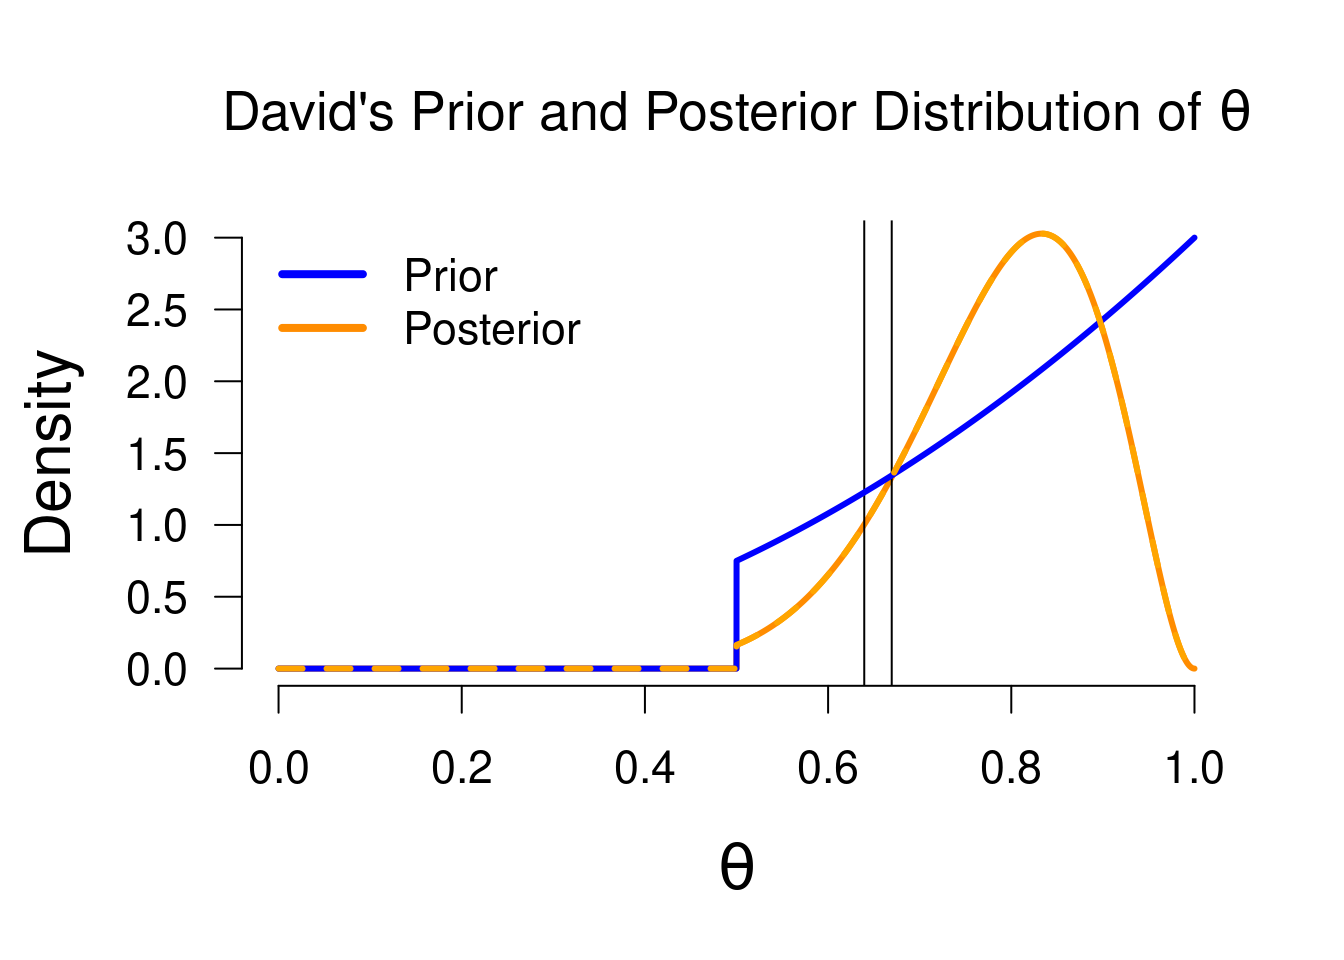
\includegraphics[width=0.9\linewidth]{_main_files/figure-latex/prior-posterior-binomial-david-1} 

}

\caption{Prior and posterior distribution for David. Values that predicted the data better than average have received a boost in plausibility (i.e., posterior density > prior density), whie the reverse holds for values that predicted the data poorly.}\label{fig:prior-posterior-binomial-david}
\end{figure}

\hypertarget{prior-distribution-in-bayesian-parameter-estimation}{%
\section{Prior Distribution in Bayesian Parameter Estimation}\label{prior-distribution-in-bayesian-parameter-estimation}}

We have now seen three different posterior distributions, for the three people (and their different prior beliefs) under consideration so far. As we have seen, the posterior distribution of Sarah is identical to her prior distribution, since she was so convinced about \(\theta = 0.5\). The posterior distributions for David and Alex are pretty similar, although not identical. This reflects a general mechanism in Bayesian parameter estimation: the more uninformed a prior distribution is, the more it lets ``the data speak for itself''. In other words, the more peaked (i.e., informed) a prior distribution is, the more data are needed to ``overthrow'' such a strong prior conviction.
In Bayesian inference for a proportion, this mechanism is neatly reflected by how the prior and posterior distribution, as well as the data, are built up. To illustrate, we can take a closer look at how we usually specify a prior distribution for a proportion.

\hypertarget{the-beta-distribution}{%
\subsection{The Beta Distribution}\label{the-beta-distribution}}

In Bayesian inference, the prior distribution can be any probability distribution (depending on which models you want to compare, or which model is most suitable for estimation). One requirement for the prior distribution is that it matches the domain of the parameter. In the case of a proportion, this means that the prior distribution ranges from 0 to 1. One such family of distributions is the \href{https://en.wikipedia.org/wiki/Beta_distribution}{\textbf{beta distribution}}. The beta distribution can take on many different shapes, based on the value of its two shape parameters \(\alpha\) and \(\beta\) (sometimes also just written in Latin, \emph{a} and \emph{b}). Setting these shape parameters changes how the beta distribution looks. You can play around in \href{https://researchmethodsuva.shinyapps.io/BayesTestMini/}{this applet} or \href{https://homepage.divms.uiowa.edu/~mbognar/applets/beta.html}{this applet}, to get an idea.

Basically, these are the dynamics:

\begin{itemize}
\tightlist
\item
  Setting \(a = b\) creates a symetric distribution, with \(a = b = 1\) giving a uniform distribution.

  \begin{itemize}
  \tightlist
  \item
    As the value of \(a = b\) increases, more and more probability mass will be centered in the middle (at 0.5), with Sarah's prior distribution as the limit (\(a = b = \infty\)).
  \end{itemize}
\item
  When \(a > b\), more probability mass will be to the right of 0.5, while the reverse holds for \(a < b\).
\item
  When \(a < 1\) and \(b < 1\), more mass will be towards the tails of the distribution (close to 0 and 1). Note that \(a\) and \(b\) need to be greater than 0.
\end{itemize}

\hypertarget{beta-interpretation-updating-section}{%
\subsection{Beta Interpretation}\label{beta-interpretation-updating-section}}

In the context of a prior distribution for a proportion, the \(a\) and \(b\) can be interpreted as previously observed heads and tails. For instance, having a uniform prior distribution (like Alex) can be seen as having observed 1 heads and 1 tails already. David's prior distribution is in fact a beta distribution with \(a = 3\) and \(b = 1\), truncated for lower values (meaning values \(< 0.5\) receive 0 probability mass). This corresponds to David having already seen 3 heads and 1 tails. In order to obtain Sarah's prior distribution, we would have a beta distribution with \(a = b = \infty\), which means that Sarah believes as if she has already seen incredibly many heads and tails.

In addition to the prior distribution, the posterior distribution for \(\theta\) is also a beta distribution. Specifically, it is a beta distribution where \(a\) is equal to the \(a\) of the prior distribution, plus the number of observed succeses/heads. The \(b\) is equal to the \(b\) of the prior distribution, plus the number of observed failures/tails. For instance, Alex' posterior distribution (Figure \ref{fig:prior-posterior-binomial}) is a beta distribution with \(a = 1 + 8 = 9\), and \(b = 1 + 2 = 3\), while David's posterior distribution (Figure \ref{fig:prior-posterior-binomial-david}) is a (trunctated) beta distribution with \(a = 3 + 8 = 11\), and \(b = 1 + 2 = 3\). Representing the knowledge updating in terms of the beta distribution also illustrates how Sarah's prior and posterior distribution are the same: her posterior \(a\) is equal to \(\infty + 8 = \infty\), and her posterior \(b\) is equal to \(\infty + 2 = \infty\).

\hypertarget{two-sided-vs-one-sided-estimation}{%
\subsection{Two-sided vs One-sided Estimation}\label{two-sided-vs-one-sided-estimation}}

Typically, when applying Bayesian estimation, we use the most uninformed model, since this model has the least bias in it. In addition, a two-sided model is generally used because the one-sided model can give misleading estimates in case it predicts the wrong side. For instance, if the true value of \(\theta\) equals 0.2, David will never assign any posterior mass to it, no matter the evidence. If we imagine observing 10 tails and 1 heads, David's posterior distribution will look as follows:

\begin{figure}

{\centering 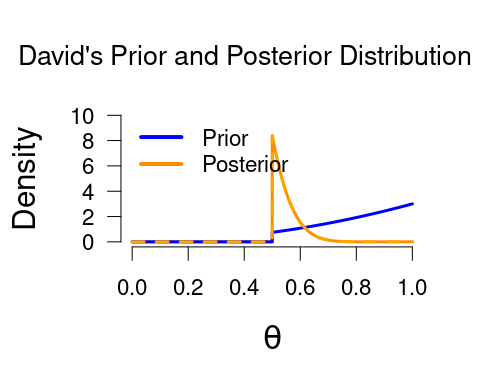
\includegraphics[width=0.9\linewidth]{_main_files/figure-latex/prior-posterior-binomial-david-alt-1} 

}

\caption{Prior and posterior distribution for David, now with 10 tails and 1 heads. This illustrates how a one-sided model can give misleading estimates: the posterior median and credible interval here will still favor values greater than 0.5, even though the data give quite some evidence for lower values.}\label{fig:prior-posterior-binomial-david-alt}
\end{figure}

While we can still take a 95\% credible interval from this posterior, it is clear that it gives a misleading estimate (the 95\% CI here will be from 0.5 to 0.65) . Since David's model only considers values between 0.5 and 1, the values that receive a boost in plausibility are those values as close as possible to the observed proportion (\(1/11\) = 0.091), so all posterior mass ``piles up'' at its truncation threshold. A two-sided model has a lot more flexibility and will simply follow along in the direction that the observed proportion is in (greater or smaller than 0.5).

\hypertarget{an-endless-loop}{%
\subsection{An Endless Loop}\label{an-endless-loop}}

What would happen if tomorrow we gather the same people again, and collect a new set of data? On this new day, they will have prior distributions equal to the posterior distributions of today, ready for a new round of knowledge updating. As more and more data accumulate (either spread over multiple days, or updated all at once), the starting prior distribution grows less influential. However, the stronger/informed the prior, the longer this process takes.

\hypertarget{relation-to-hypothesis-testing}{%
\section{Relation to Hypothesis Testing}\label{relation-to-hypothesis-testing}}

So far we have been talking about models. In order to conduct a hypothesis test, we can take several of these models and compare their predictive performance through the Bayes factor (see section \ref{model-comparison-section} and section \ref{more-model-comparison-section}). Typically, the model with extreme conviction about a ``null value''\footnote{The null value is typically the value that implies no effect, such as 0.5 for a proportion, or 0 for a correlation or t-test.}, which in this case would be Sarah's model. Then, what we call the alternative hypothesis can be any other model that corresponds to the theory one wants to test: all models we have seen so far make some specific statement about plausible values of \(\theta\). The Bayes factor simply tells us which model predicted the data the best: it is a relative metric that compares two models at a time.

\hypertarget{the-savage-dickey-density-ratio}{%
\subsection{The Savage-Dickey Density Ratio}\label{the-savage-dickey-density-ratio}}

When employing such a null/alternative hypothesis setup, there exists a convenient computational trick to obtain the Bayes factor of one alternative model over the null model. When we take the updating of the alternative model, for instance Alex', we can take the prior density at the value of testing (\(0.5\)) and the posterior density at the value of testing. The ratio of these two values is equal to the Bayes factor comparing Alex and Sarah's models. The prior density at 0.5 equals 1 (i.e.~\(P(\theta = 0.5) = 1\)) and the posterior density at 0.5 equals approximately 0.5 (i.e., (\(P(\theta = 0.5 \mid \text{data}) \approx 0.5\))), so their ratio is approximately \(1 / 0.5 = 2\), in favor of the alternative hypothesis (i.e., \(\text{BF}_{10} \approx 2\)). The Savage-Dickey density ratio also implies the following: when the prior density is higher than the posterior density at the value of testing, we will find evidence in favor of the alternative hypothesis (the magnitude of evidence depends on how much lower the prior density is). This makes sense: the value of testing is the only value that is considered by the null hypothesis, so if that value has suffered a \emph{decline} in plausibility as a result of the data, then that means the null hypothesis as a whole did not do well. Figure \ref{fig:prior-posterior-binomial-sd-ratio} below shows Alex' prior and posterior distribution, with the grey dots indicating the density ratio.

For a different point of testing, for instance \(0.8\), we can take the Savage-Dickey density ratio at that point. With a test value of 0.8, the null model becomes equal to Paul's model (his prior distribution was concentrated on the value 0.8), so we are comparing Alex' model to Paul's model. In Figure \ref{fig:prior-posterior-binomial-sd-ratio}, the density values are indicated by the purple dots. Here, the null model (i.e., Paul's model) did very well, since \(0.8\) fits the observed data very well, as indicated by the posterior density being much higher than the prior density at that point (\(\text{BF}_{01} \approx 3\)).

\begin{figure}

{\centering 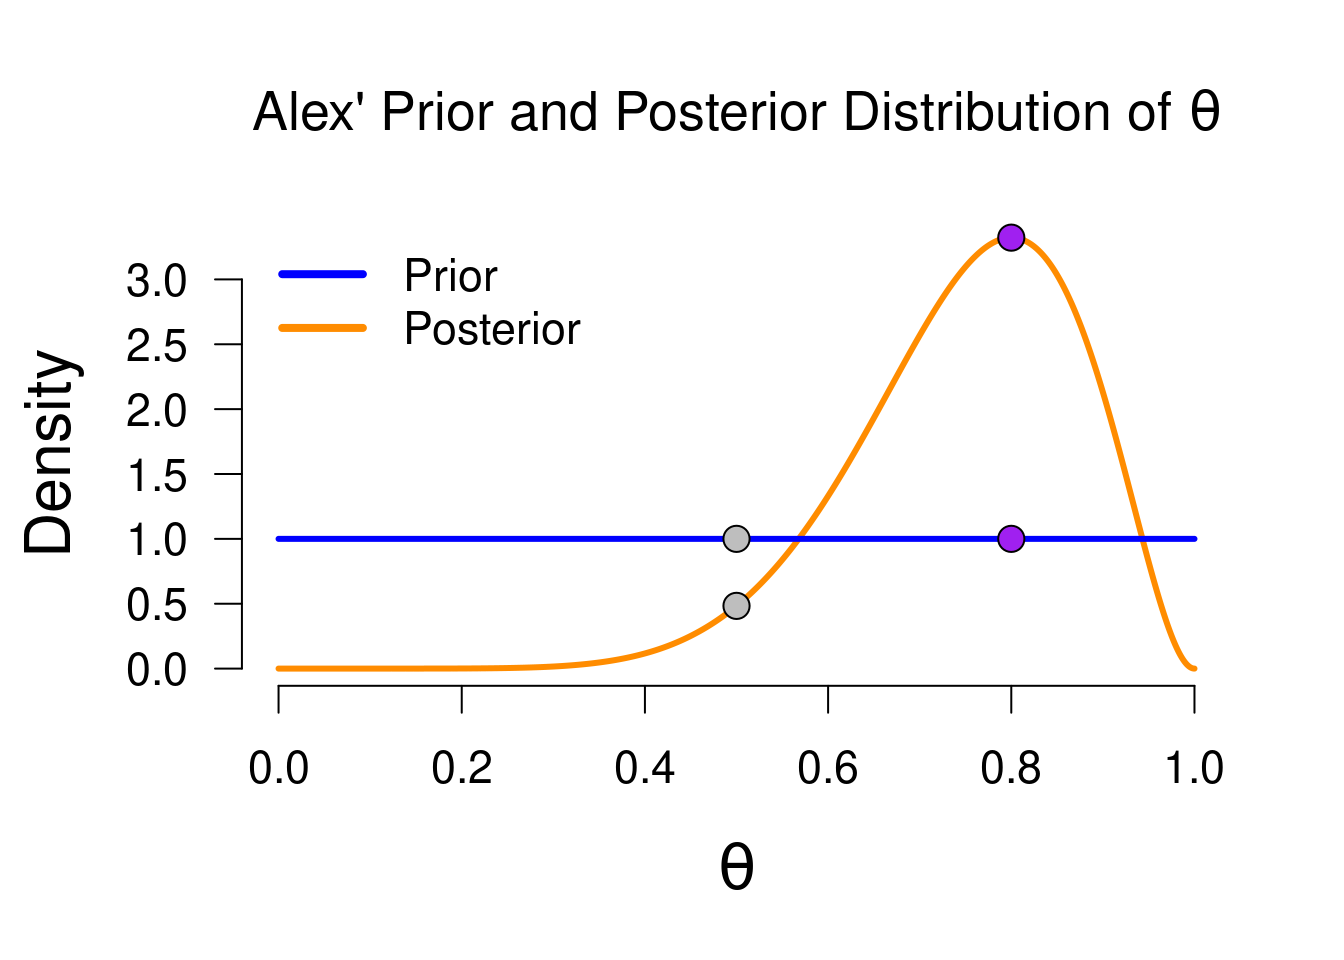
\includegraphics[width=0.9\linewidth]{_main_files/figure-latex/prior-posterior-binomial-sd-ratio-1} 

}

\caption{Prior and posterior distribution for Alex, with the grey/purple dots indicating the prior/posterior density values for two test values: 0.5 and 0.8. The ratio of the grey values is equal to the Bayes factor comparing Alex' and Sarah's models, while the ratio of the purple values is equal to the Bayes factor comparing Alex' and Paul's models. This ratio is known as the Savage-Dickey density value.}\label{fig:prior-posterior-binomial-sd-ratio}
\end{figure}

\hypertarget{concluding-thoughts-1}{%
\section{Concluding Thoughts}\label{concluding-thoughts-1}}

In this chapter, we have seen how different models learn from the same data to form posterior beliefs. These posterior beliefs about the parameter can then be used to make an estimation (i.e., a probabilistic statement) of the parameter in the form of a \(x\%\) Credible Interval, or posterior median.

We have seen several key ideas:

\begin{itemize}
\tightlist
\item
  Prior knowledge (i.e., what a model believes, \emph{before} seeing the data) is characterized by a probability distribution: in the case of proportion \(\theta\), we typically use the beta distribution
\item
  Prior knowledge is then updated with the updating factor, which consists of the likelihood of the observed data, and the average likelihood for that model
\item
  Values of \(\theta\) that predicted the data well will receive a boost in plausibilty (posterior density \textgreater{} prior density) and values that predicted the data poorly will receive a penalty in plausibilty (prior density \textgreater{} posterior density)
\item
  The posterior distribution reflects our posterior knowledge (i.e., what a model believes, \emph{after} seeing the data), which we use to make an estimate of the parameter
\item
  Strong prior convictions will need more data to be overthrown.
\end{itemize}

\hypertarget{the-beer-tasting}{%
\chapter{The Beer Tasting}\label{the-beer-tasting}}

With several key components of Bayesian inference explained, we can return to the beer tasting. Just as before, we have several models at our disposal that make certain claims about the proportion \(\theta\). In this case, \(\theta\) is the population proportion of people that will give the correct response to which of the two beers contains alcohol. Again, a model can be extremely convinced of \(\theta\) being equal to a single value, such as \(0.5\), which implies that people are simply guessing (i.e., the null hypothesis). Alternatively, a model can spread its prior beliefs by using the beta distribution. This beta distibution can then be two-sided (if the model wants to bet on all values between 0 and 1), or truncated to be one-sided (if the model only wants to bet on values greater \textbf{or} smaller than 0.5). These models can function as the alternative hypothesis. We will use these models for hypothesis testing, which is just another term for model comparison. In this chapter, we will analyze the beer tasting results from a Bayesian point of view, to get a practical understanding of the concepts introduced in the previous chapters.

\hypertarget{methods}{%
\section{Methods}\label{methods}}

On a Friday afternoon, May 12th 2017, an informal beer tasting experiment took place at the Psychology Department of the University of Amsterdam. The experimental team consisted of three members: one to introduce the participants to the experiment and administer the test, one to pour the drinks, and one to process the data. Participants tasted two small cups filled with Weihenstephaner Hefeweissbier, one with alcohol and one without, and indicated which one contained alcohol. Participants were also asked to rate the confidence in their answer (measured on a scale from \(1\) to \(100\), with \(1\) being completely clueless and \(100\) being absolutely sure), and to rate the two beers in tastiness (measured on a scale from \(1\) to \(100\), with \(1\) being the worst beer ever and \(100\) being the best beer ever).
The experiment was double-blind, such that the person administering the test and interacting with the participants did not know which of the two cups contained alcohol. For ease of reference, each cup was labeled with a random integer between \(1\) and \(500\), and each integer corresponded either to the alcoholic or non-alcoholic beer. A coin was flipped to decide which beer was tasted first.
The setup was piloted with \(9\) participants; subsequently, we tested as many people as possible within an hour, and also recorded which of the two beers was tasted first. On average, testing took approximately 30 seconds per participant, yielding a total of \(57\) participants. Of the 57 participants, 42 (\(73.7\%\)) correctly identified the beer that contained alcohol: in other words, there were \(s = 42\) successes and \(f = 15\) failures.\footnote{Three video recordings of the procedure are available at \url{https://osf.io/428pb/}}

\hypertarget{analysis-in-jasp}{%
\section{Analysis in JASP}\label{analysis-in-jasp}}

In order to analyze the collected data in JASP, the Bayesian binomial test can be used, which can be found under the menu labeled ``Frequencies''. Several settings are available for the binomial test, allowing exploration of different analysis choices. Figure \ref{fig:jasp-screenshot-binomial-test} presents a screenshot of the options panel in JASP. For this analysis, we specify a test value of \(0.5\) (i.e., chance performance), and \(a = b = 1\) for the prior distribution of \(\theta\) under \(\mathcal{H}_1\). Note that in a sensitivity or robustness analysis (covered in the next chapter), other values for \(a\) and \(b\) may be explored to assess their impact on the posterior distribution.

\begin{figure}

{\centering 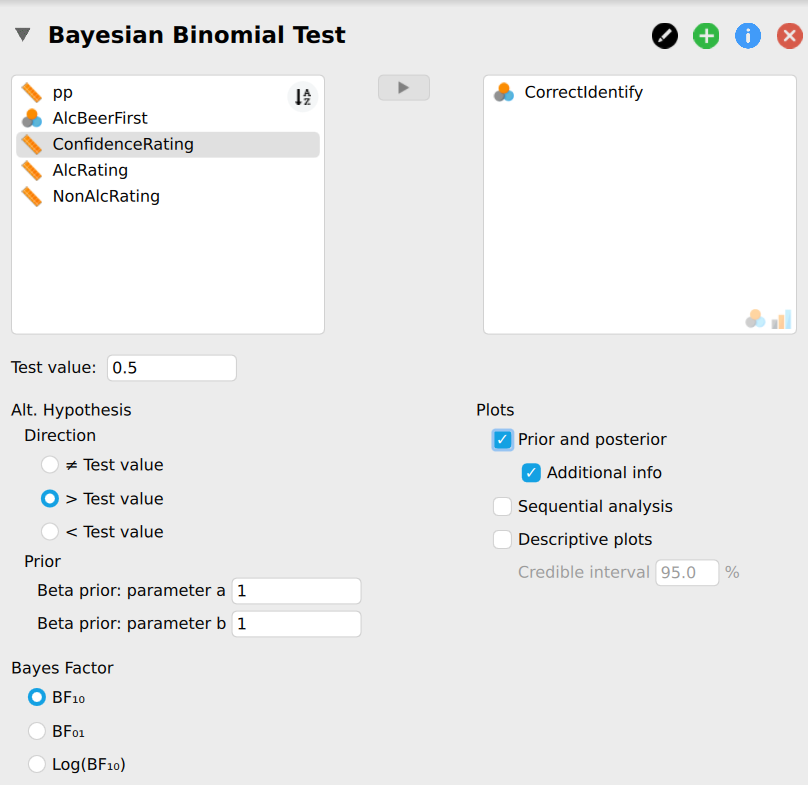
\includegraphics[width=1\linewidth]{Figures/binomTestJASPpanel2022} 

}

\caption{Screenshot of the options for the Bayesian binomial test in JASP.}\label{fig:jasp-screenshot-binomial-test}
\end{figure}

The null hypothesis here postulates that participants perform at chance level, which implies \(\theta = 0.5\) since if participants cannot taste the difference, they will just be guessing. The alternative hypothesis postulates that this is not the case. There are several options for the alternative hypothesis in terms of \(a\), \(b\), and its directionality. For instance, in the case of two-sided hypothesis testing, the hypotheses can be specified as follows:
\begin{equation*}
\mathcal{H}_0:  \theta = 0.5
\end{equation*}
\begin{equation}
\mathcal{H}_1:  \theta \sim \text{beta}(1, 1)\text{.}
\label{eq:hypoSetupTwoSided}
\end{equation}
However, since we wish to test whether or not participants' discriminating ability \emph{exceeds} chance, we can specify the alternative hypothesis to allow only values of \(\theta\) greater than \(0.5\) (note the `\(+\)' in the subscript):
\begin{equation}
\mathcal{H}_+:  \theta \sim \text{beta}(1, 1) \text{I}  (0.5, 1)\text{,}
\label{eq:hypoSetup}
\end{equation}
where I indicates truncation of the beta distribution to the interval \([0.5, 1]\).

Figure \ref{fig:jasp-beer-result} illustrates the results of the binomial test. The left panel shows the prior and the posterior distribution of \(\theta\) for the \textbf{two-sided alternative hypothesis}, along with the median and credible interval of the posterior distribution. The posterior median equals \(0.731\) and the \(95\%\) credible interval ranges from \(0.610\) to \(0.833\), indicating a substantial deviation of \(\theta\) from \(0.5\). For each value of \(\theta\), the change from prior distribution to posterior distribution is quantified by predictive adequacy: for those values of \(\theta\) that predict the data better than average, the posterior density exceeds the prior density. Additionally, the two-sided Bayes factor \(\text{BF}_{10} = 112\), which means the data are 112 times more likely under \(\mathcal{H}_1\) than under \(\mathcal{H}_0\).

The right panel shows inference for the \textbf{one-sided positive hypothesis} (i.e., \(\mathcal{H}_+: \theta \geq 0.5\)) compared to the null hypothesis: the resulting Bayes factor is \(225.26\) in favor of the alternative hypothesis, which means the data are \(225\) times more likely under \(\mathcal{H}_+\) than under \(\mathcal{H}_0\).
Note that the posterior distribution itself has hardly changed, compared to the two-sided result: the posterior median still equals \(0.731\) and the \(95\%\) credible interval ranges from \(0.610\) to \(0.833\).
Because virtually all posterior mass was already to the right of \(0.5\) in the two-sided case, the posterior distribution was virtually unaffected by changing from \(\mathcal{H}_1\) to \(\mathcal{H}_+\).
However, in the right panel, \(\mathcal{H}_+\) only predicts values greater than \(0.5\), which is reflected in the prior distribution: all prior mass is now located in the interval \((0.5\text{, } 1)\), and as a result, the prior mass in the interval \((0.5\text{, } 1)\) has doubled. If the posterior remains constant, but the prior mass doubles, this means that the Bayes factor also doubles (perhaps best illustrated by the Savage-Dickey density ratio).
In other words, a model that is predicting the data well and is focusing more on those values (e.g., \(\mathcal{H}_+\)) has more evidence in its favor than a model that is predicting the data well, but spread its bets more (e.g., \(\mathcal{H}_1\)). Such a built in reward for making a more specific prediction is an important mechanism in Bayesian model comparison, and is known as \textbf{parsimony}. Making a more specific prediction comes with a risk though: \(\mathcal{H}_-\) predicted the data a lot worse than \(\mathcal{H}_0\) because it bet on the wrong direction.

\begin{figure}

{\centering 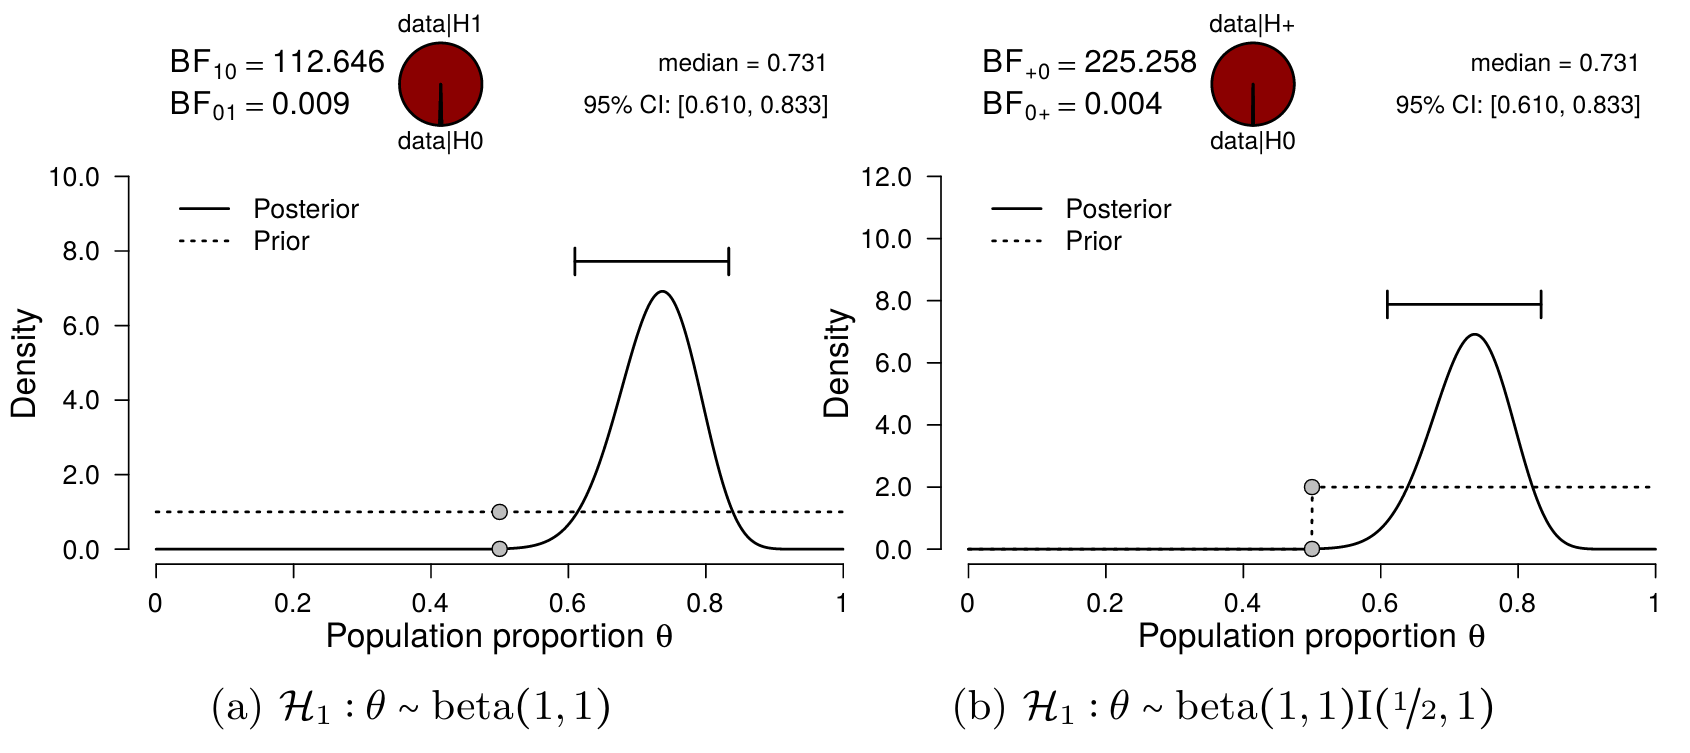
\includegraphics[width=0.95\linewidth]{Figures/beerTasteResultsPriorPostOneTwoSided} 

}

\caption{Bayesian binomial test for theta. The probability wheel at the top illustrates the ratio of the evidence in favor of the two hypotheses. The two gray dots indicate the Savage-Dickey density ratio. The median and the 95 percent credible interval of the posterior distribution are shown in the top right corner. The left panel shows the two-sided test and the right panel shows the one-sided test.}\label{fig:jasp-beer-result}
\end{figure}

\hypertarget{continuous-updating}{%
\section{Continuous Updating}\label{continuous-updating}}

The beer tasting experiment also highlights one of the main strengths of Bayesian inference: real-time monitoring of the incoming data. As the data accumulate, the analysis can be continuously updated to include the latest results. In other words, the results may be updated after every participant, or analyzed all at one, without affecting the resulting inference. To illustrate this, we can compute the posterior distribution for the first \(9\) participants of the experiment for which \(s = 6\) and \(f = 3\). Specifying the same beta prior distribution as before, namely a truncated beta distribution with shape parameters \(a = b = 1\), and combining this with the data, yields a truncated beta posterior distribution with shape parameters \(a = 6 + 1 = 7\) and \(b = 3 + 1 = 4\) (see also Section \ref{beta-interpretation-updating-section}).\footnote{ 
The shape parameters of the beta posterior distribution can be obtained by summing the $a$ and $b$ parameters of the prior distribution with the observed number of successes and failures, respectively.} The resulting posterior distribution is presented in the left panel of Figure \ref{fig:jasp-beer-result-updating}. Now, we can take the remaining 48 participants and update our knowledge once more. Because we already have knowledge about the population's rate parameter \(\theta\), namely the results of the first 9 participants, we can incorporate this in the analysis through the prior distribution, following Lindley's maxim ``today's posterior is tomorrow's prior'' \citep{Lindley1972}.

In this case, we start with a truncated beta prior distribution with \(a = 7\) and \(b = 4\), and update this with the data of the remaining 48 participants. Out of the 48 participants, 36 were correct, and 12 were incorrect. Updating the prior distribution with this data yields a posterior distribution with shape parameters \(a = 7 + 36 = 43\) and \(b = 4 + 12 = 16\), which is exactly the same posterior distribution obtained when analyzing the full data set at once. This two-step procedure is illustrated in Figure \ref{fig:jasp-beer-result-updating}. The left panel shows the original prior distribution (i.e., the truncated beta distribution with \(a = 1, b = 1\)) and the posterior distribution for the first \(9\) participants. The right panel shows the inference for the remaining \(48\) participants, while starting with the posterior-turned-prior distribution reflecting the knowledge about the first \(9\) participants (a truncated beta distribution with \(a = 7, b = 4\)).

\begin{figure}

{\centering 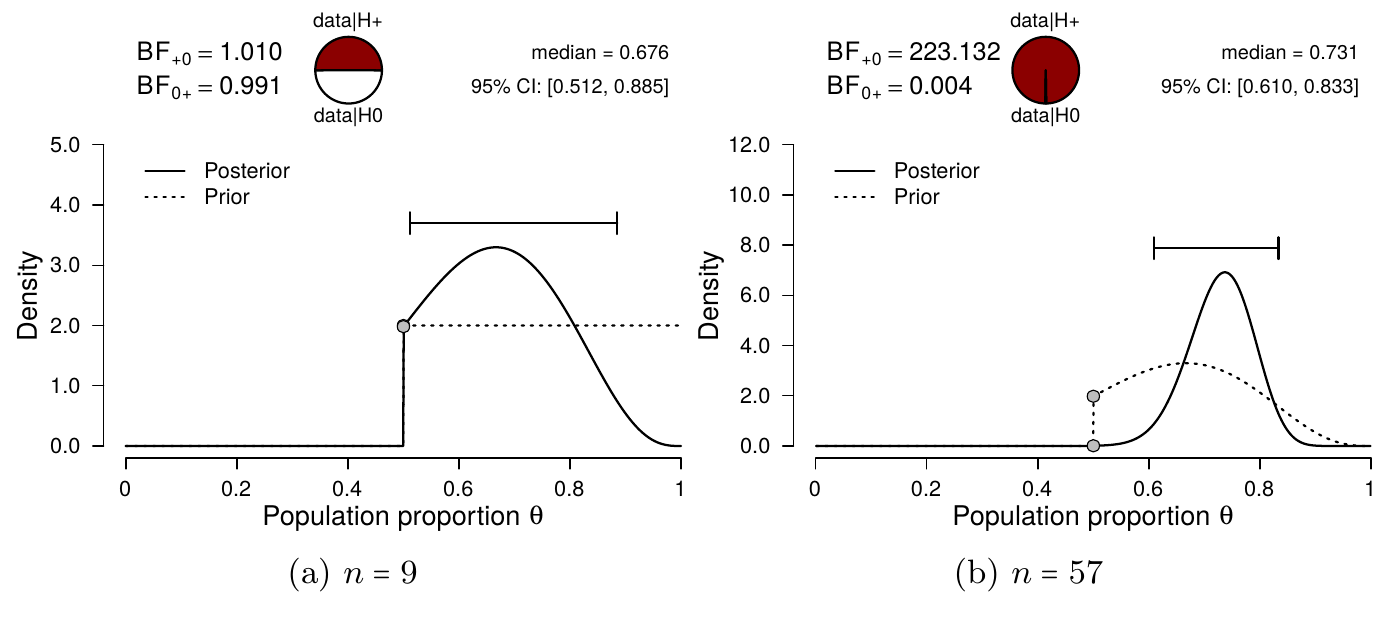
\includegraphics[width=1\linewidth]{Figures/BeerUpdatingPosteriorPlot} 

}

\caption{Sequential updating of the Bayesian binomial test. The left panel shows results from a one-sided Bayesian binomial test for the first $n = 9$ participants ($s = 6$, $f = 3$). The shape parameters of the truncated beta prior were set to $a = 1$ and $b = 1$. The right panel shows results from a one-sided binomial test for the remaining $48$ participants. Here, the specified prior is the posterior distribution from the left panel: a truncated beta distribution with $a+s = 7$ and $b+f = 4$.  The resulting posterior distribution is identical to the posterior distribution in Figure 4.2. In order to obtain the total Bayes factor in Figure 4.2 (i.e., 225), the component Bayes factors from the left and right panel can be multiplied: $1.01 * 223 = 225$.}\label{fig:jasp-beer-result-updating}
\end{figure}

We can even look at the evolution of the Bayes factor, as the data come in. This development can be inspected by means of a \textbf{sequential analysis}. Figure \ref{fig:jasp-beer-result-updating} shows the evolution of the Bayes factor as more data are collected. Initially the evidence is inconclusive, but after about \(30\) participants the evidence increasingly supports \(\mathcal{H}_1\). Being able to monitor the data as such can be very useful while planning or conducting an experiment. For instance, instead of needing to already commit to a certain sample size, a researcher can simply keep going untill a certain evidence threshold (for either hypothesis) is reached.\footnote{This is in contrast to using \(p\)-values, where the data can only be analyzed once, and any additional look at the data will inflate the type I error rate.}

\begin{figure}

{\centering 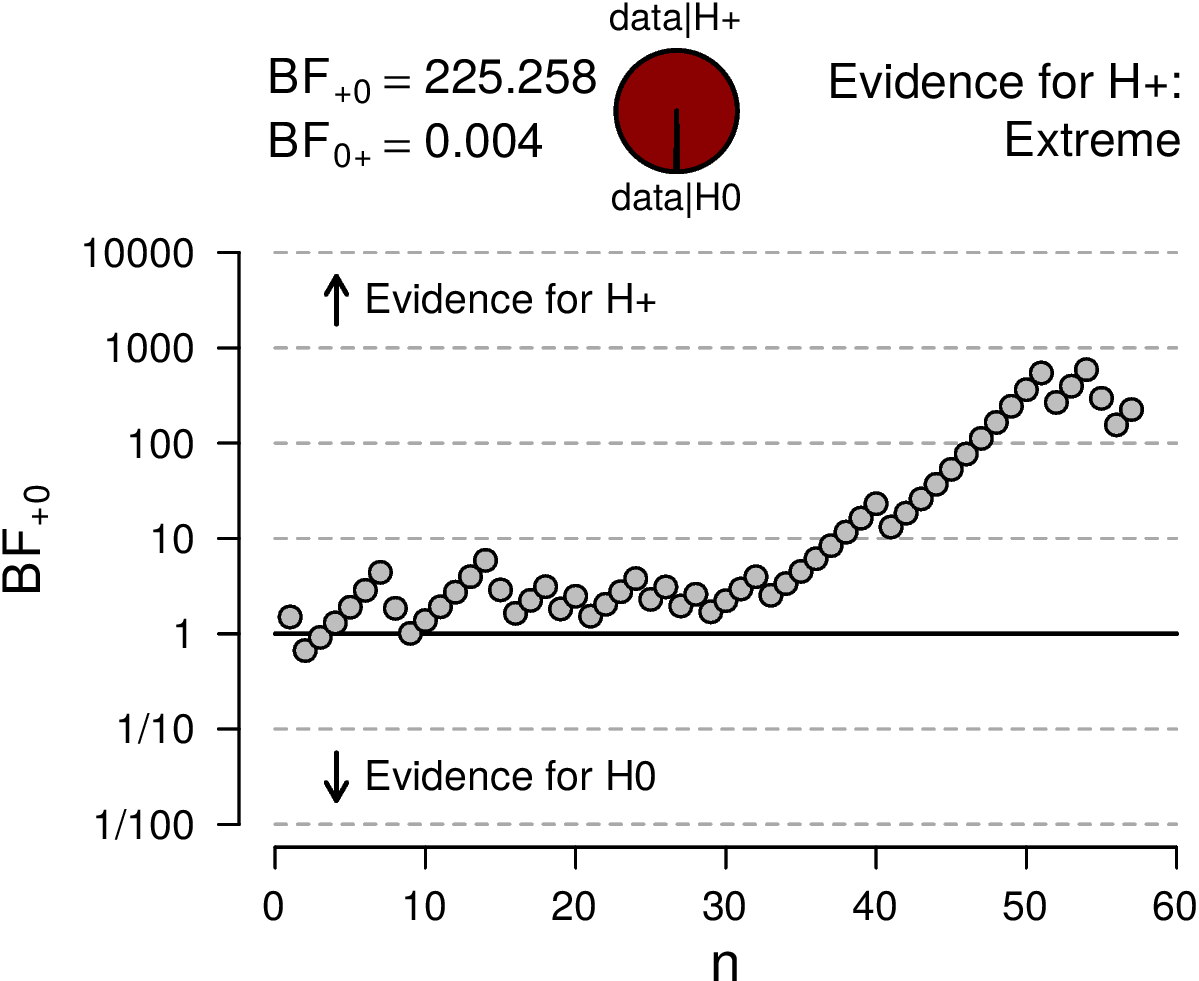
\includegraphics[width=1\linewidth]{Figures/BeerSequentialAnalysis} 

}

\caption{Sequential analysis, showing the evolution of the Bayes factor as $n$, the number of observed participants, increases. After an initial period of relative inconclusiveness, the Bayes factor strongly favors $H_+$.}\label{fig:jasp-beer-result-sequential-analysis}
\end{figure}

\hypertarget{concluding-thoughts-2}{%
\section{Concluding Thoughts}\label{concluding-thoughts-2}}

In this chapter we compared several models that made a statement about the beer tasting ability of people. The null model was absolutely sure that people cannot taste the difference between alcoholic and non-alcoholic beer, while the positive alternative model (\(\mathcal{H}_+\)) stated that people's ability ranges uniformly from 0.5 to 1. The Bayes factor comparing the predictions of \(\mathcal{H}_+\) and \(\mathcal{H}_0\) indicated the observed proportion, \(0.73\) (\(n = 57\)), to be 225 times more likely under \(\mathcal{H}_+\) than under \(\mathcal{H}_0\). This can be seen as very strong evidence (see Figure \ref{fig:bayes-factor-classification}) in favor of the theory that people can taste the difference between the two beers. In addition, Bayesian knowledge updating was illustrated by analyzing the data sequentially, as opposed to all at once.

\hypertarget{more-bayesian-analyses}{%
\chapter{More Bayesian Analyses}\label{more-bayesian-analyses}}

All of the concepts that were discussed in the previous chapters can also be applied to Bayesian analyses for other types of research questions, such as correlations or differences in means (i.e., the \(t\)-test). In the current chapter, we will explore these tests using the same beer-tasting data set. Besides measuring whether participants identified the correct beer, we also recorded how tasty they found each of the two beers, which we can use to answer the following two questions:

\begin{itemize}
\tightlist
\item
  Do people find alcoholic beer tastier?
\item
  Is there an association between tastiness ratings?
\end{itemize}

\hypertarget{the-bayesian-t-test}{%
\section{The Bayesian T-Test}\label{the-bayesian-t-test}}

The first question, ``do people find alcoholic beer tastier?'', concerns the difference between means. Since each participant tasted the alcoholic and non-alcoholic beer, this was measured within subjects, and so a within subjects \(t\)-test is required. For Bayesian \(t\)-tests, the parameter of interest is denoted \(\delta\) (``delta''). This parameter is a standardized difference between two means, and is formally known as ``Cohen's \emph{d}'', a very common \href{https://en.wikipedia.org/wiki/Effect_size}{effect size} in psychology.\footnote{There are many more effect sizes that can quantify a difference in means, but for simplicity's sake we focus on Cohen's \emph{d} here.} When doing inferential statistics, we can either estimate the magnitude of this effect size, conduct model comparison, or both. In the sections below, the Bayesian ingredients are described for the \(t\)-test.

\hypertarget{prior-distribution}{%
\subsection{Prior Distribution}\label{prior-distribution}}

The prior distribution is always defined on the same domain as the parameter of interest. For the proportion, this was the convenient domain of {[}0, 1{]}, and so allowed the use of the beta distribution, and the possibility to use the uniform distribution as the uninformed prior distribution. The domain of \(\delta\) instead goes from \(-\infty\) to \(\infty\), so its prior distribution has to match that domain. For a nulhypothesis this does not matter so much, since the null hypothesis generally posits a single value (e.g., 0, stating there is no difference between the groups). However, for the alternative hypothesis it becomes tricky now to have a uniform distribution on the whole domain of \(\delta\). Since the domain is infinitely big, the density of a uniform distribution between \(-\infty\) and \(\infty\) would need to be infinitely small, which is not very practical. Instead, what is generally done is to apply a probability distribution that is spread out a little less (although still a lot more than a point null hypothesis). One such distribution is the \href{https://en.wikipedia.org/wiki/Cauchy_distribution}{Cauchy distribution}, which is a \(t\) distribution with a single degree of freedom. The width of the Cauchy distribution is determined by the \textbf{Cauchy scale parameter}. Below, several examples are given:

\begin{figure}

{\centering 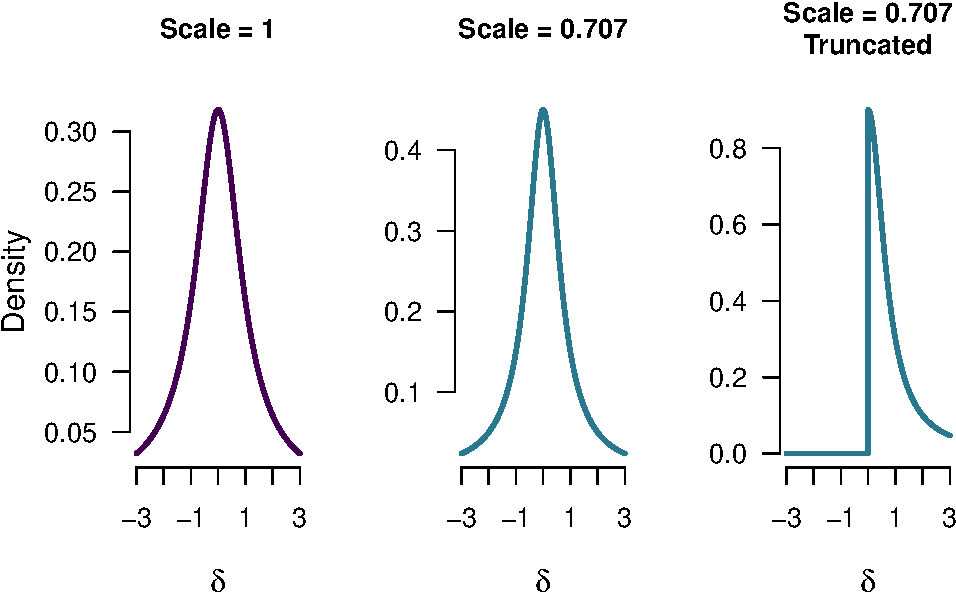
\includegraphics[width=1\linewidth]{_main_files/figure-latex/three-cauchy-dists-1} 

}

\caption{Three different Cauchy distributions. Each of these can be used as a model for the difference between two groups, and each of these has a (slightly) different theoretical implication.}\label{fig:three-cauchy-dists}
\end{figure}

Just as before, these distributions can serve as a statement about the population parameter. Also just as before, each of these models make predictions about the world, and will have a certain quality of their prediction: how well did they predict the data? We can look at how well they did, and compare it to how well the null model (which went ``all-in'' on 0) predicted the data. Before we do that, we can first take a look at how these models will learn from the data: how is this prior knowledge updated to form posterior knowledge?

\hypertarget{predictive-updating-factor}{%
\subsection{Predictive Updating Factor}\label{predictive-updating-factor}}

The Bayesian belief updating again follows the general form presented in Section \ref{model-estimation-section}. Again, we update the prior knowledge with information from the data. In the case of the beer tasting experiment, there was an observed effect size of \(0.714\) (for more descriptives see Figure \ref{fig:beer-tastiness-descriptives} below).

\begin{figure}

{\centering 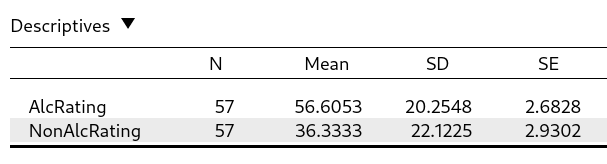
\includegraphics[width=1\linewidth]{Figures/DescriptivesBeerTastiness} 

}

\caption{The descriptive statistics for the tastiness ratings for both the alcoholic and non-alcoholic beers. The observed mean for the alcoholic beer is higher than for the non-alcoholic beer, but how much evidence is there in favor of this difference?}\label{fig:beer-tastiness-descriptives}
\end{figure}

The predictive updating factor quantifies how well each of the values in the model predicted the observed effect of \(0.714\) (as quantified by the likelihood), compared to how well the model did on average (as quantified by the marginal likelihood). Figure \ref{fig:beer-t-test-likelihood} below shows the likelihood of the observed data for various values of \(\delta\). The purple bar indicates the marginal likelihood for the one-sided Cauchy model (scale = 0.707), to show which values in that model will receive a boost in plausibility. Remember that it is the likelihood function that is the same for any model, but that the marginal likelihood of that model will differ (based on its predictions).

\begin{figure}

{\centering 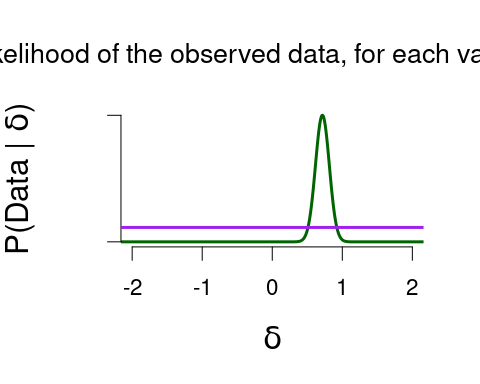
\includegraphics[width=1\linewidth]{_main_files/figure-latex/beer-t-test-likelihood-1} 

}

\caption{The likelihood of the observed data, for various values of delta. The higher the likelihood, the better that value predicted the data.}\label{fig:beer-t-test-likelihood}
\end{figure}

\hypertarget{posterior-distribution-bayes-factor}{%
\subsection{Posterior Distribution \& Bayes Factor}\label{posterior-distribution-bayes-factor}}

Values in the model that predicted the data well, will see in increase in density when comparing prior to posterior distribution. \ref{fig:beer-t-test-likelihood} shows that values between 0.5 and 1 will receive a boost in plausibility. Figure \ref{fig:beer-tastiness-t-test-posterior} below shows the JASP-results for the Bayesian \(t\)-test, using a one-sided alternative hypothesis to test the hypothesis that people like the alcoholic beer more than the non-alcoholic beer. The posterior distribution is fairly concentrated between \(0.5\) and \(1\), with a 95\% credible interval from 0.398 to 0.978, so that is already some evidence that the tastiness ratings differ between the two beers. In addition, the Bayes factor comparing the predictions of the two hypotheses shows that the data are 22200 times more likely under the alternative hypotheis \(\mathcal{H}_{+}\) than under \(\mathcal{H}_{0}\).

\begin{figure}

{\centering 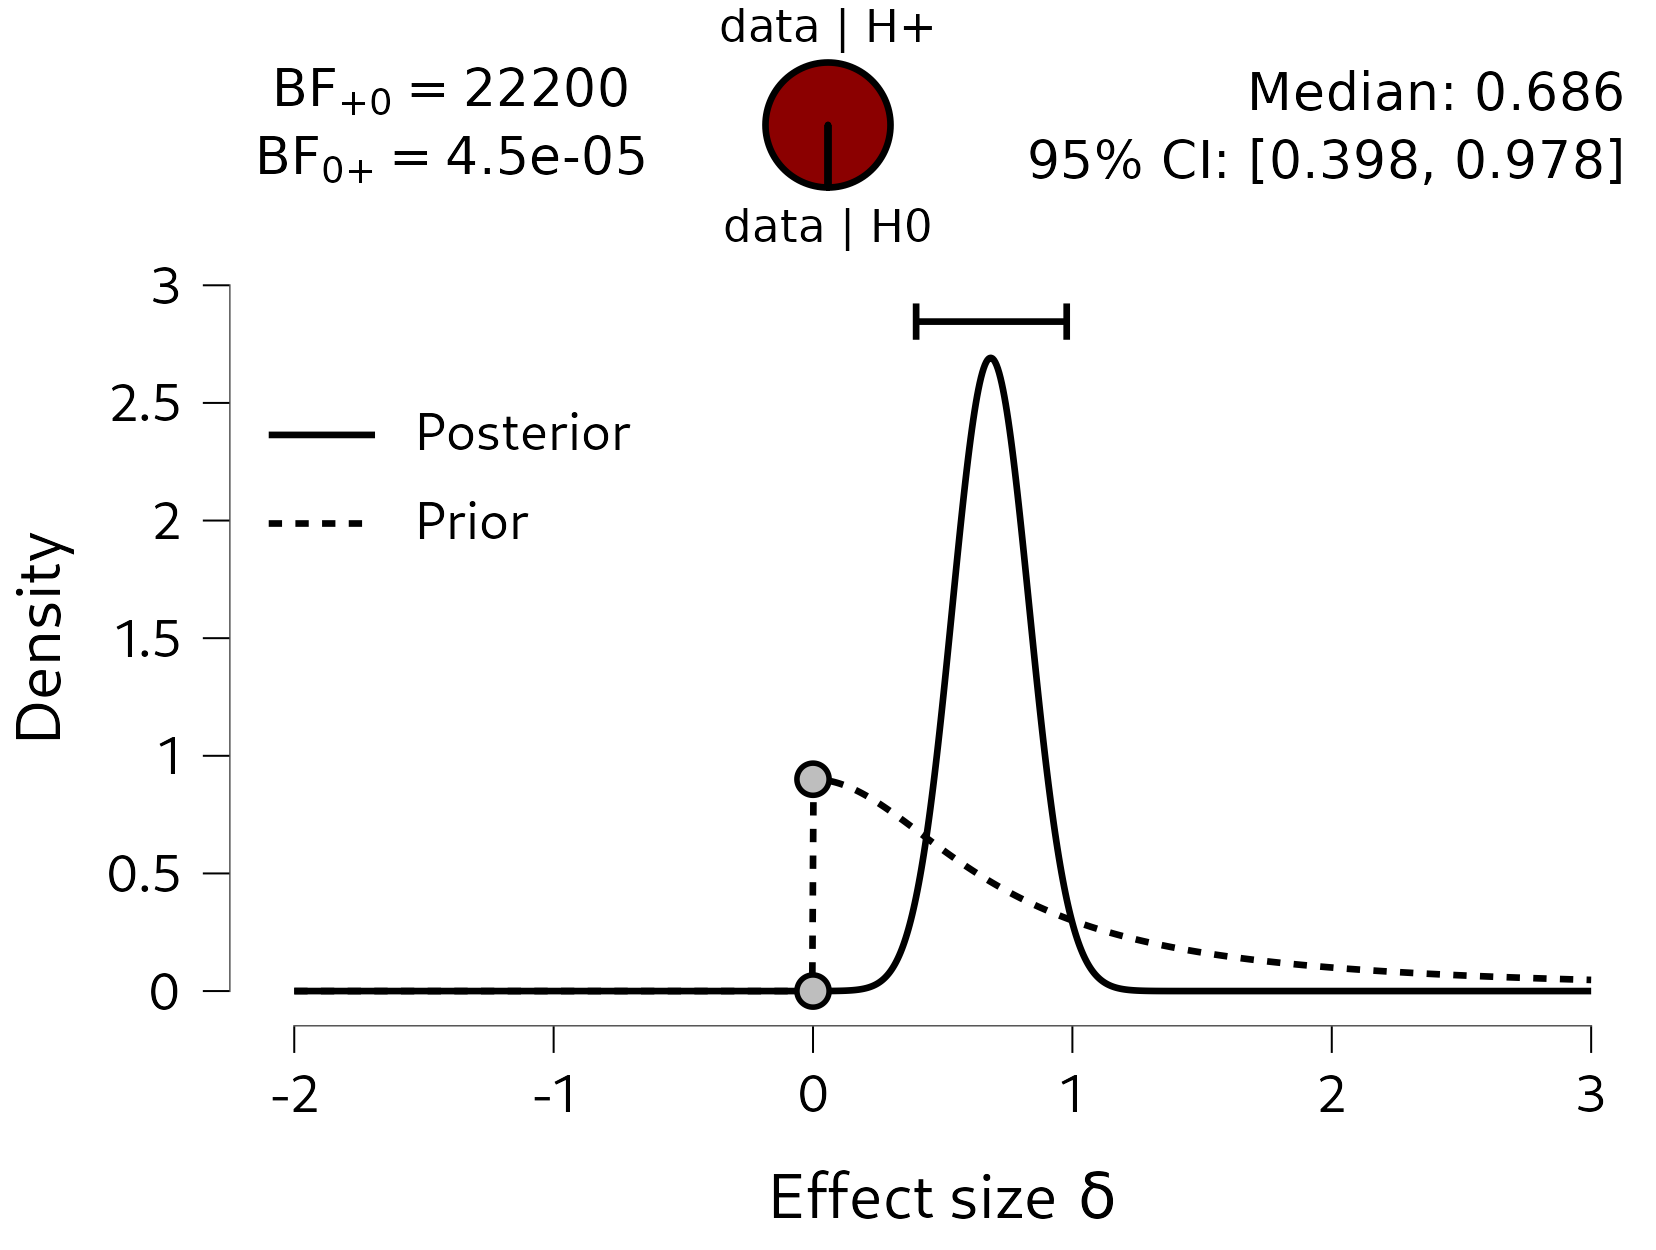
\includegraphics[width=1\linewidth]{Figures/TTestBeerTastiness} 

}

\caption{The results of the Bayesian paired samples t-test on the tastiness ratings. The bayes factor comparing the predictions of the one-sided, positive, alternative hypothesis to the null hypothesis is very strongly in favor of the alternative hypothesis:  the data are 22200 times more likely under the alternative hypothesis than under the null hypothesis.}\label{fig:beer-tastiness-t-test-posterior}
\end{figure}

\hypertarget{bayes-factor-robustness}{%
\subsubsection{Bayes Factor Robustness}\label{bayes-factor-robustness}}

Specifying the prior distribution is a fairly subjective endeavor in Bayesian analyses. For most analyses, there exist some guiding principles for choosing an uninformative prior distribution, but it is still worth investigaing how robust the obtained Bayes factor is to different prior specifications. Since the Bayes factor compares the predictions of two models, changing the prior distribution changes the model's prediction and therefore also alters the Bayes factor. To analyze to what extent this happens, a \textbf{robustness check} can be conducted, where different prior specifications are explored.

For the \(t\)-test, where the Cauchy prior distribution is governed by a single shape parameter (its scale), a convenient plot can be constructed, where the Bayes factor is shown as a function of the shape parameter. Figure \ref{fig:beer-tastiness-t-test-robustness} shows such a plot. Here we can see that there is quite strong evidence in favor of \(\mathcal{H}_{+}\) for almost all Cauchy prior widths in the graph (i.e., the line is relatively flat). Only for extreme values of the Cauchy scale parameter (around \(0.05\)), does the evidence in favor of \(\mathcal{H}_{+}\) decrease towards 1. This is a logical consequence of changing the prior distribution: the prior distribution formalizes a model's predictions, and if the prior distribution becomes extremely narrow, it starts resembling the null model. For a Cauchy width of, say, \(0.01\), the alternative and null model make very similar predictions, and so the Bayes factor will be around 1. In the context of a robustness check, we can ignore such extreme specifications. We generally aim to detect whether, for instance, the Bayes factor with a width of 1 qualitatively differs from the Bayes factor with a width of 0.5. If that is the case, then our result is perhaps not so reliable, and we would need more data to create a more robust result.

\begin{figure}

{\centering 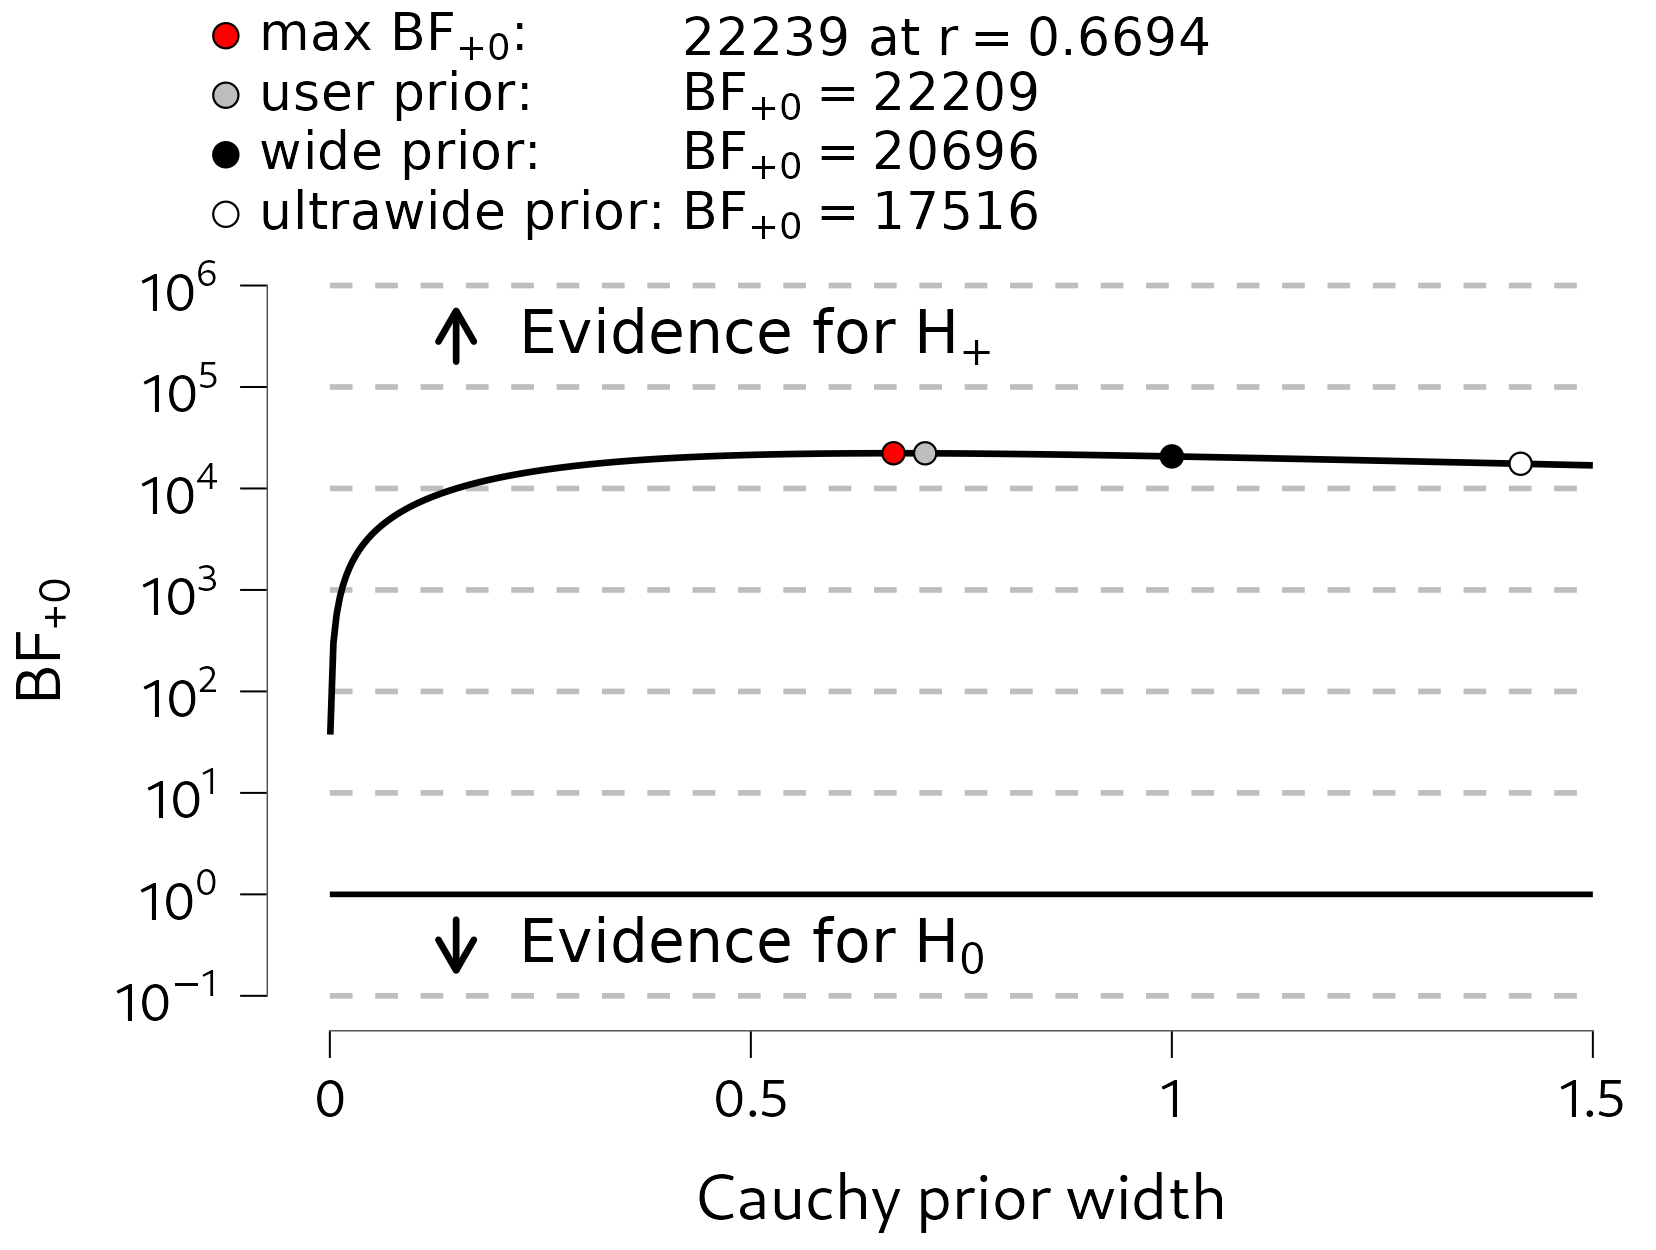
\includegraphics[width=0.9\linewidth]{Figures/TTestBeerTastinessRobustness} 

}

\caption{A robustness analysis of the Bayesian t-test. Here we explore how much the Bayes factor changes, as a result of using a different value for the Cauchy scale parameter. Generally, the flatter the line, the more robust the Bayes factor is to different prior specifications.}\label{fig:beer-tastiness-t-test-robustness}
\end{figure}

\hypertarget{the-bayesian-correlation}{%
\section{The Bayesian Correlation}\label{the-bayesian-correlation}}

In addition to testing whether there is a difference in tastiness ratings, we can also analyze whether there is an association between the ratings of the two beers: are people who rate the alcoholic beer as tasty, more inclined to also rate the non-alcoholic beer as tasty? In other words, are there people who just really like Weihenstephaner (and give both beers high scores), and people who do not (and give both beers low scores)?

In order to do so, we can conduct a Bayesian correlation analysis. We will again be using all the key ingredients from the previous chapters. We will start with some prior distribution, then update this with the information in the observed data, to form posterior knowledge about the population correlation \(\rho\) (``rho''). Additionally, we can conduct a hypothesis test, where we compare a model that states no association between the ratings, and a model that states that there is some positive association.

To conduct a Bayesian correlation test in JASP, you can select (after loading the data) ``Regression'', then ``Bayesian correlation''. This presents the correlation analysis for several variables. To obtain more results, you can go to ``Plot Individual Pairs'', where JASP allows a more thorough analysis of individual pairs of variables. See Figure \ref{fig:beer-tastiness-correlation-JASP} for a screenshot of the current analysis.

\begin{figure}

{\centering 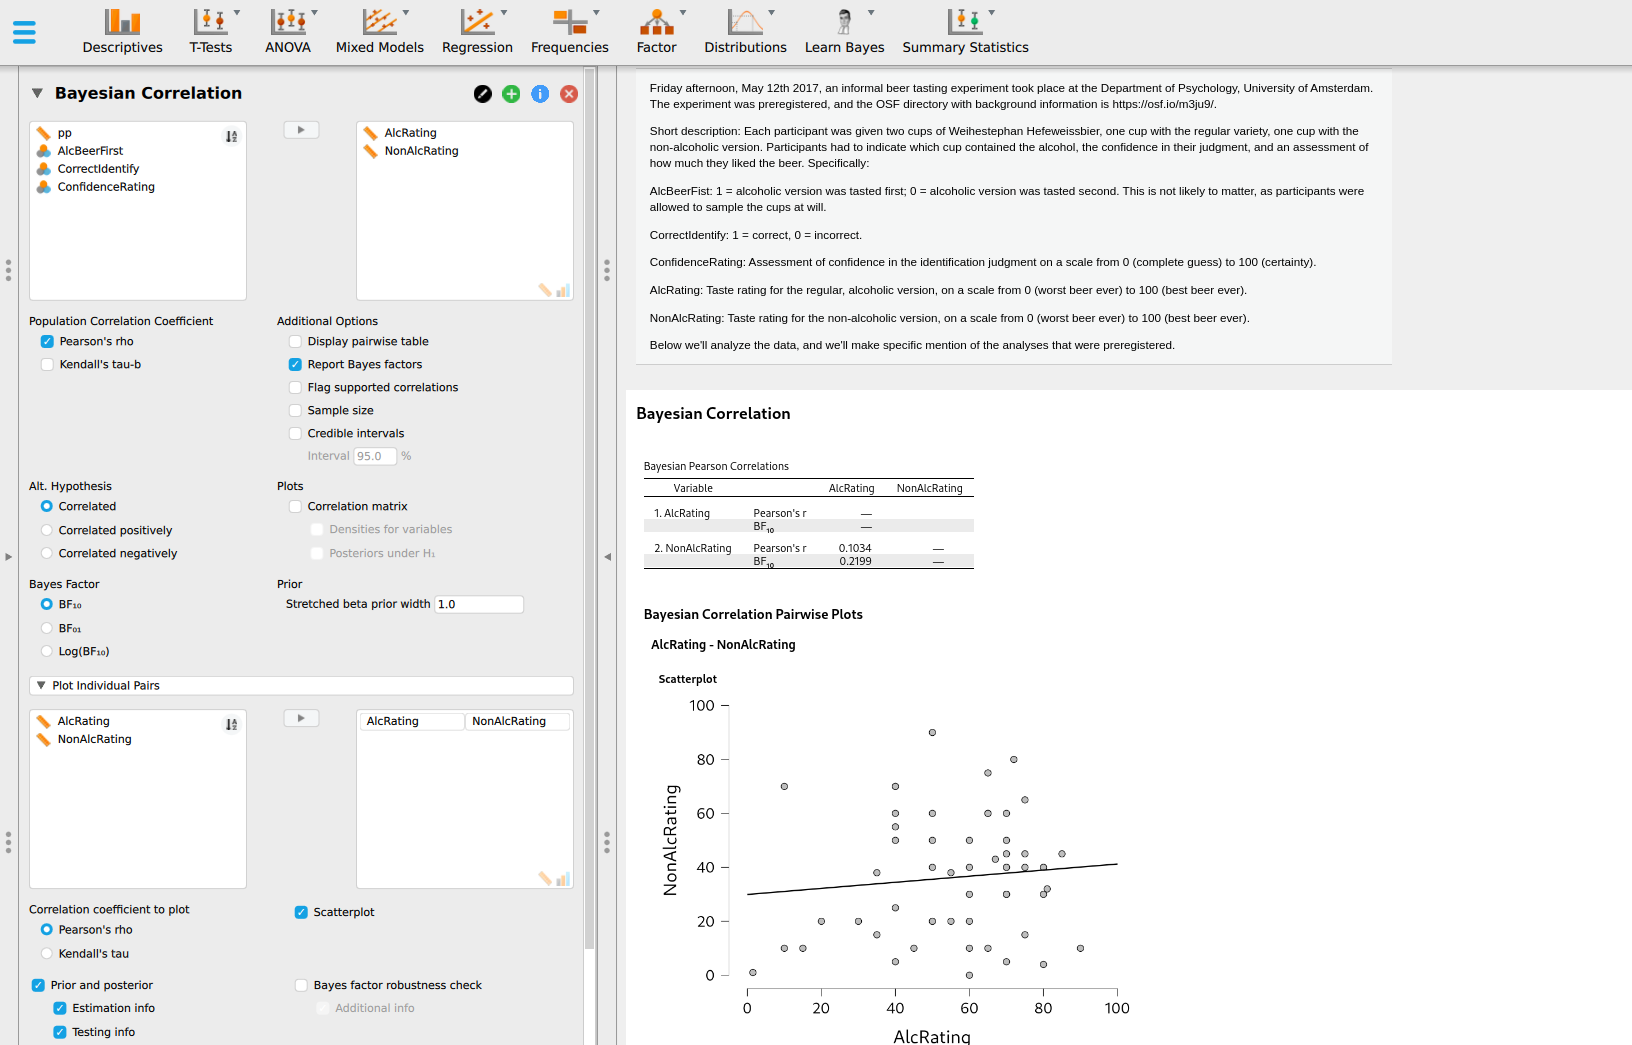
\includegraphics[width=0.9\linewidth]{Figures/correlationTestJASPpanel2022} 

}

\caption{The JASP user interface for the Bayesian correlation analysis. To enable more analysis options, the "Plot Individual Pairs" tab can be used.}\label{fig:beer-tastiness-correlation-JASP}
\end{figure}

\hypertarget{prior-distribution-1}{%
\subsection{Prior Distribution}\label{prior-distribution-1}}

The domain of the correlation is \([-1, 1]\), so we a prior distribution that matches that domain. In this case, we can take the beta distribution from before, and stretch its domain to create the \textbf{stretched beta distribution}. While before, the values of a and b can be specified individually, for the stretched beta distribution we only set a single value for both a and b: the prior width. The width is the inverse of \(a\) and \(b\): a width equal to 0.5 means a stretched beta distribution with \(a\) and \(b\) equal to \(1 / 0.5 = 2\). A width equal to 1 means a stretched beta distribution with \(a = b = 1\). Figure \ref{fig:three-stretched-beta-dists} shows three versions of the stretched beta distribution - additionally showing that these distributions can also be one-sided (i.e., only considering negative or positive correlations).

\begin{figure}

{\centering 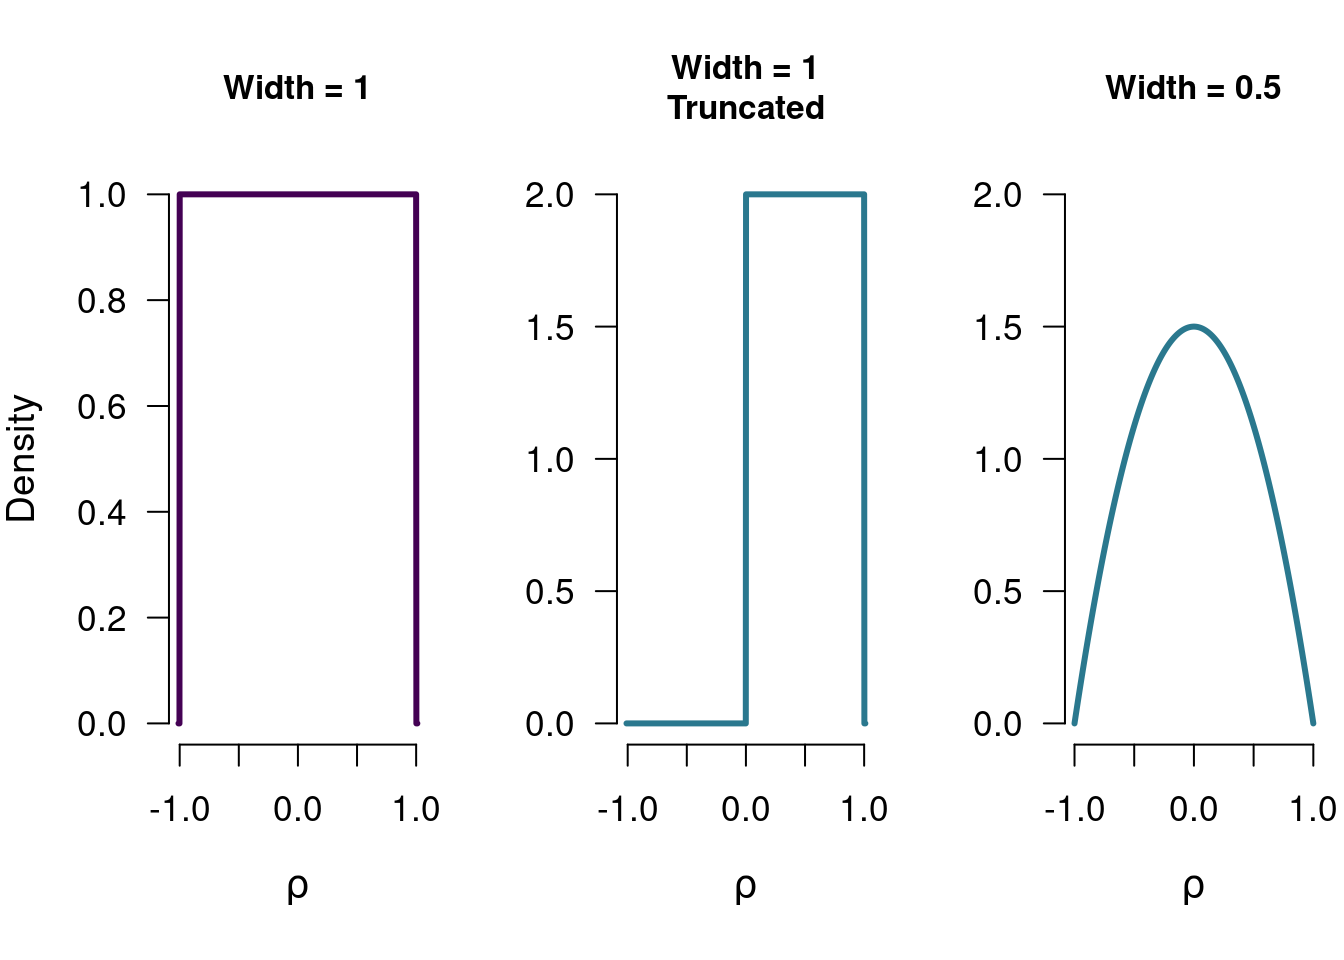
\includegraphics[width=1\linewidth]{_main_files/figure-latex/three-stretched-beta-dists-1} 

}

\caption{Three different stretched beta distributions. Each of these can be used as a model for the correlation, and each of these has a (slightly) different theoretical implication.}\label{fig:three-stretched-beta-dists}
\end{figure}

\hypertarget{predictive-updating-factor-1}{%
\subsection{Predictive Updating Factor}\label{predictive-updating-factor-1}}

The observed correlation \(r\) is equal to \(0.1034\), and we can look at how likely this result is for various values of the population correlation \(\rho\). Figure \ref{fig:beer-correlation-likelihood} shows the likelihood function. The likelihood of observing a correlation of \(0.1\) is highest when the population correlation is in fact equal to \(0.1\). As before, the likelihood illustrates which values of \(\rho\) have a good match (i.e., a good prediction) with the observed data.

To see which values in the model predicted the data better than average, we can look at the marginal likelihood for that model. The purple bar in Figure \ref{fig:beer-correlation-likelihood} shows the marginal likelihood for the two-sided model (prior width = 1). We use the marginal likelihood to see which values of \(\rho\) deserve a boost in plausibilty, and later we will compare marginal likelihoods of different models to obtain a Bayes factor.

\begin{figure}

{\centering 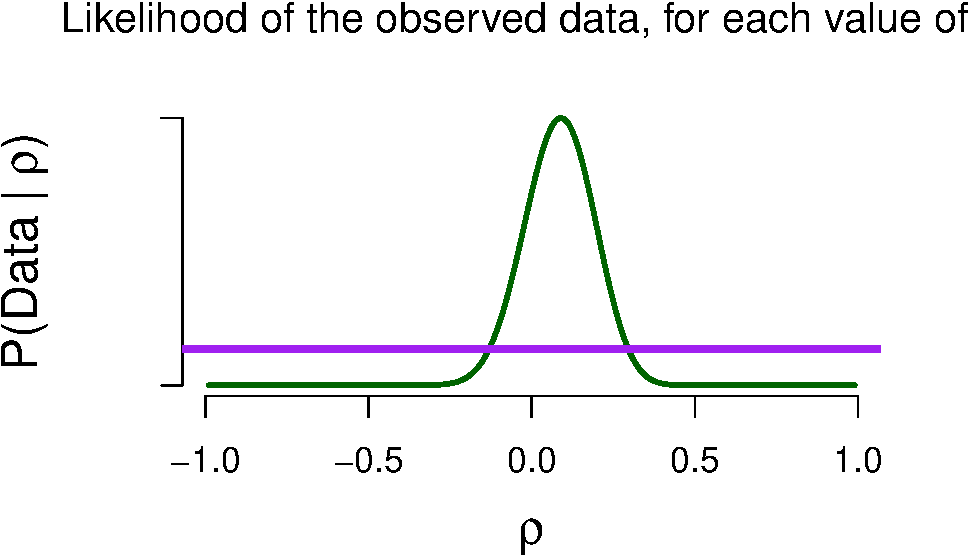
\includegraphics[width=1\linewidth]{_main_files/figure-latex/beer-correlation-likelihood-1} 

}

\caption{The likelihood of the observed data, for various values of rho. The higher the likelihood, the better that value predicted the data. The likelihood is the highest for the observed correlation (0.1).}\label{fig:beer-correlation-likelihood}
\end{figure}

\hypertarget{posterior-distribution-bayes-factor-1}{%
\subsection{Posterior Distribution \& Bayes Factor}\label{posterior-distribution-bayes-factor-1}}

The updated beliefs about \(\rho\) are shown in Figure \ref{fig:beer-tastiness-correlation-posterior}. In order to test whether there is an association, we can look at the Bayes factor. Here, we have found moderate evidence in favor of the null hypothesis: the data are 4.5 times more likely under the null model, compared to the alternative model. This highlights an important feature of Bayesian hypothesis testing: since we concretely quantify what both models predict, we can actually obtain evidence \emph{in favor} of the null hypothesis. This means we can distinguish between \textbf{absence of evidence} and \textbf{evidence of absence}. The former means that there is just no evidence to conclude that there is an association, while the latter means that we have found evidence for the lack of an association. In terms of Bayes factors, absence of evidence occurs when we observe a Bayes factor close to 1 (no evidence either way), while evidence of absence occurs when we observe \(\text{BF}_{01} > 1\).
The evidence in favor of the null also highlights the Savage-Dickey density ratio: \(\rho\) being equal to 0 has become more plausible as a result of the data (its posterior density is greater than its prior density). This means that models that bet a lot of money on this value (such as the null model) will do very well in model comparisons.

In terms of parameter estimation, we can look at the posterior median and credible interval. The posterior median is quite close to 0, and the 95\% credible interval ranges from \(-0.158\) to \(0.3436\): under the two-sided uniform model, there is a 95\% probability that the true value of \(\rho\) lies in that interval.

\textbackslash begin\{figure\}

\{\centering 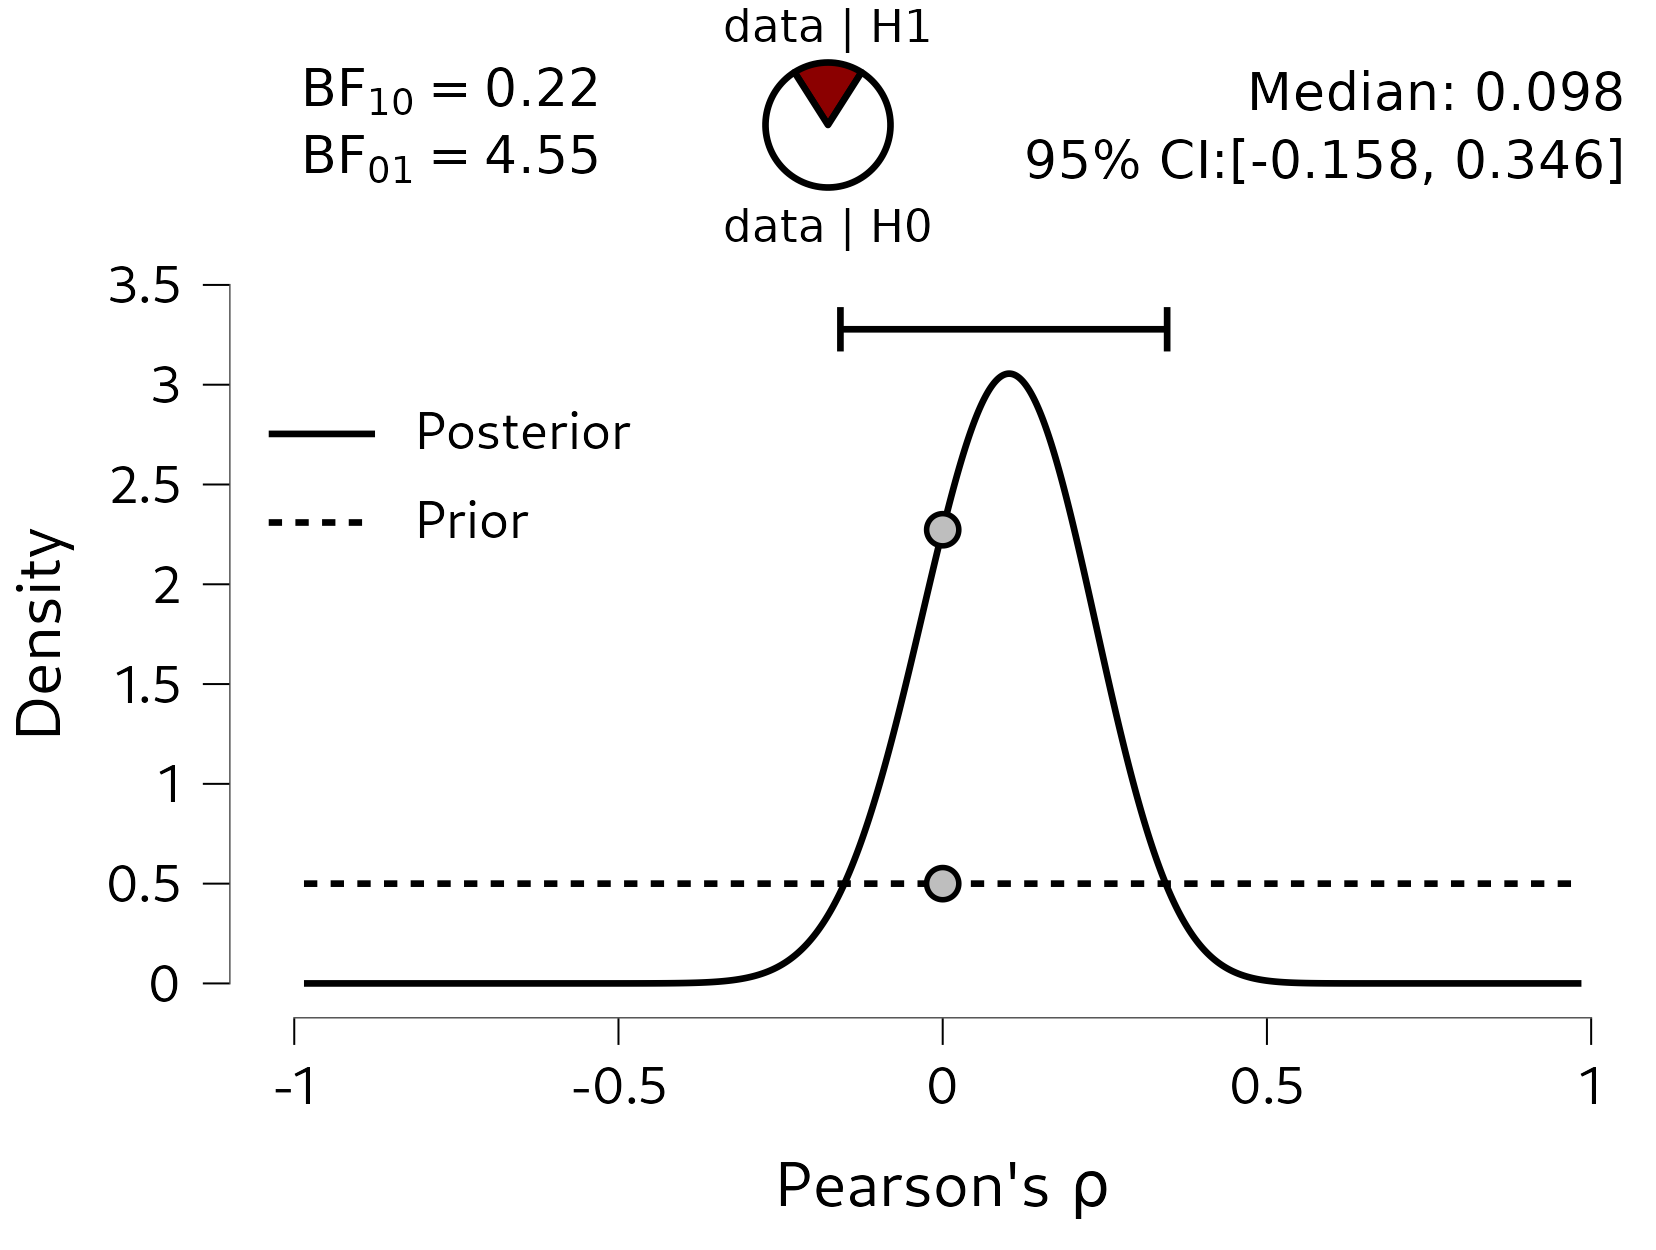
\includegraphics[width=1\linewidth]{Figures/CorrelationTestPosterior}

\}

\textbackslash caption\{The posterior distribution of rho, based on a two-sided uniform prior distribution. Under this model, there is a 95\% probability that rho is between -0.155 and 0.331. There is moderate evidence in favor of the null hypothesis: the data are 4.5 times more likely under the null model, compared to the alternative model.\}\label{fig:beer-tastiness-correlation-posterior}
\textbackslash end\{figure\}

\hypertarget{concluding-thoughts-3}{%
\section{Concluding Thoughts}\label{concluding-thoughts-3}}

In this chapter, we have seen the Bayesian concepts from the previous chapters, but then applied to different research questions/parameters. Instead of models making statements about \(\theta\), we looked at parameters that govern a difference between means (\(\delta\)) or an association (\(\rho\)). With a different parameter comes a different type of prior distribution, since the prior distribution matches the domain of the parameter. However, everything that follows is exactly the same as for the binomial analysis: the prior distribution is updated using the (marginal) likelihood to form posterior beliefs. We can compare marginal likelihoods of different models to obtain a Bayes factor. To investigate the robustness of the Bayes factor to the choice of prior distribution, a robustness check can be conducted.

Lastly, the Bayes factor helps to distinguish between ``evidence of absence'' and ``absence of evidence''. This is quite informative, since they have two distinct meanings. Traditionally in psychology, journals are mostly interested in ``non-null'' effects, since these are deemed a lot sexier (and also because the p-value cannot easily distinguish between EoA and AoE). This results in some stress for empirical researchers: what if you spent 2 years of your PhD project collecting data, and you do not find your hypothesized effect and therefore cannot publish? Being able to quantify evidence in favor of the null hypothesis can hopefully create a scientific discourse that is more inclusive towards null-findings.

\hypertarget{exercises}{%
\chapter{Exercises}\label{exercises}}

Below you will find various exercises on the intricate world of Bayesian inference, testing your knowledge and intuition about Bayesian parameter estimation and Bayesian hypothesis testing in the context of various statistical tests (binomial test, correlation, \(t\)-test). The exercises use statistical software JASP (\url{https://jasp-stats.org}). Each exercise lists links to webpages with either only JASP output (so you can also complete the exercises without installing JASP), or with annotated JASP output containing the solutions/explanation to the exercises (and additional ramblings that hopefully provide some extra intuition). The output files can also be found here in case the OSF does not work for you: \url{https://surfdrive.surf.nl/files/index.php/s/OHjXsc79TkeYWgN}

If you want to conduct an analysis in JASP, but get stuck, you can consult \href{https://youtube.com/playlist?list=PLWPa8RxHarcOyxhMAk_RMT9h_GYHCrgGQ}{this playlist with 3 instructional videos (one for each of the analyses below)}

\hypertarget{binomial-test}{%
\section{Binomial Test}\label{binomial-test}}

\hypertarget{therapeutic-touch}{%
\subsection{Therapeutic Touch}\label{therapeutic-touch}}

Therapeutic Touch (TT) is a nursing practice rooted in mysticism but alleged to have a scientific basis. Practitioners of TT claim to treat medical conditions by using their hands to manipulate a ``human energy field'' perceptible above the patients' skin. Being a skeptical mind, 9-year old Emily Rosa ventured to test these claims by designing an experiment where TT practitioners had to correctly identify the location of the experimenter's hand (above their left or right hand) while being blinded by a screen. The results of this experiment were later published in the prestigious Journal of the American Medical Association (Rosa et al., 1998). In the following exercise, you will evaluate this data set with JASP.

\begin{itemize}
\tightlist
\item
  JASP file with only the results: \url{https://osf.io/snu9r/}
\item
  JASP file with results and interpretation/solutions: \url{https://osf.io/273yp/}
\end{itemize}

\begin{enumerate}
\def\labelenumi{\arabic{enumi}.}
\tightlist
\item
  Open the ``Emily Rosa'' dataset from the JASP Data Library (you can find it in the folder ``Frequencies''). Alternatively, use the link above to view the results without using JASP.
\item
  Get a descriptive overview of the data by producing a frequency table of the variable Outcome (Go to ``Frequencies'', then ``Bayesian Binomial Test'' and select the variable ``Outcome''). How many practitioners guessed correctly? What is the proportion?
\item
  Produce a prior and posterior plot for a two-sided test and interpret the 95\% credible interval displayed in it.
\item
  Conduct a Bayesian Binomial Test to test if the practitioners' ability (i.e., proportion of correct responses) is better than random (i.e., \(\theta > 0.5\)). Use the default prior for the alternative hypothesis. What is the Bayes factor in favor of the null hypothesis (\(\text{BF}_{0+}\))?
\item
  How would you interpret the Bayes factor?
\item
  Take a look at the sequential analysis plot. What was (approximately) the largest Bayes factor in favor of the alternative hypothesis that was ever reached in the sequential analysis of the data?
\item
  Imagine a previous experiment with 10 practitioners, where 8 therapists gave the correct answer. Construct an informed prior distribution based on their results. How do the results of the hypothesis test change when compared to a default prior?
\end{enumerate}

\hypertarget{psychologists-tasting-beer}{%
\subsection{Psychologists Tasting Beer}\label{psychologists-tasting-beer}}

Friday afternoon, May 12th 2017, an informal beer tasting experiment took place at the Department of Psychology, University of Amsterdam. The experiment was preregistered, the OSF directory with background information is \url{https://osf.io/m3ju9/}, and the corresponding article can be found at \url{https://psyarxiv.com/d8bvn/}.

Short description: Each participant was (blinded) given two cups of Weihestephan Hefeweissbier, one cup with the regular variety, one cup with the non-alcoholic version. Participants had to indicate which cup contained the alcohol, the confidence in their judgment, and an assessment of how much they liked the beer. The data set contains the following variables:

\begin{itemize}
\tightlist
\item
  AlcBeerFist: 1 = alcoholic version was tasted first; 0 = alcoholic version was tasted second. This is not likely to matter, as participants were allowed to sample the cups at will.
\item
  CorrectIdentify: 1 = correct, 0 = incorrect.
\item
  ConfidenceRating: Assessment of confidence in the identification judgment on a scale from 0 (complete guess) to 100 (certainty).
\item
  AlcRating: Taste rating for the regular, alcoholic version, on a scale from 0 (worst beer ever) to 100 (best beer ever).
\item
  NonAlcRating: Taste rating for the non-alcoholic version, on a scale from 0 (worst beer ever) to 100 (best beer ever).
\end{itemize}

In this exercise, you will conduct a Bayesian binomial test to analyze the proportion of correct responses.

\begin{itemize}
\tightlist
\item
  csv file with the data: \url{https://osf.io/zh9md/}
\item
  JASP file with only the results: \url{https://osf.io/azkvc/}
\item
  JASP file with results and interpretation/solutions: \url{https://osf.io/jn3es/}
\end{itemize}

\begin{enumerate}
\def\labelenumi{\arabic{enumi}.}
\tightlist
\item
  Download the csv file from the OSF and open the data in JASP. Alternatively, use the link above to view the results without using JASP.
\item
  Get a descriptive overview of the data by producing a frequency table of the variable Outcome (go to ``Frequencies'', then ``Bayesian Binomial Test'' and select the variable ``CorrectIdentify''). What percentage of participants had a correct response (``1'')?
\item
  Which settings can we use to specify our alternative hypothesis (see Figure \ref{fig:jasp-screenshot-binomial-test} for the available settings)? What do these settings imply?
\item
  Using a uniform prior distribution, what are the two-sided Bayes factors (\(\text{BF}_{10}\)) for the proportion of incorrect responses (``0'') and for the proportion of correct responses (``1'')? Are they equal? Explain why (not).
\item
  In order to test whether people are able to taste the difference, conduct a one-sided hypothesis test to test if \(\theta > 0.5\). What is the Bayes factor (\(\text{BF}_{+0}\))? How do you interpret this? What is your verdict on the claim that psychologists can taste the difference between alcoholic and non-alcoholic beer?
\item
  Conduct a Sequential analysis to inspect how the Bayes factor developed as the data accumulated. Did it ever provide strong evidence for the null hypothesis? Around which value did the Bayes factor cross the threshold of 100?
\item
  Imagine being someone who is very confident in psychologists beer tasting ability, because they once did their own experiment and saw that 10 out of 11 could taste the difference. What would their prior distribution look like? How does this affect the one-sided Bayes factor (\(\text{BF}_{+0}\)) for the proportion of correct responses?
\end{enumerate}

\hypertarget{correlation}{%
\section{Correlation}\label{correlation}}

\hypertarget{correlation-a.w.e.s.o.m.-o-4000}{%
\subsection{Correlation: A.W.E.S.O.M.-O 4000}\label{correlation-a.w.e.s.o.m.-o-4000}}

In South Park episode 116, one of the series' main protagonists, Eric Cartman, pretends to be a robot from Japan, the ``A.W.E.S.O.M.-O 4000''. When kidnapped by Hollywood movie producers and put under pressure to generate profitable movie concepts, Cartman manages to generate thousands of silly ideas, 800 of which feature Adam Sandler. We conjecture that the makers of South Park believe that Adam Sandler movies are
profitable regardless of their quality. In this exercise, we put forward the following South Park hypothesis: ``For Adam Sandler movies, there is no correlation between box-office success and movie quality (i.e.,''freshness'' ratings on Rotten Tomatoes; www.rottentomatoes.com).''

\begin{itemize}
\tightlist
\item
  JASP file with only the results: \url{https://osf.io/xs9dq/}
\item
  JASP file with results and interpretation/solutions: \url{https://osf.io/5fq6s/}
\end{itemize}

\begin{enumerate}
\def\labelenumi{\arabic{enumi}.}
\tightlist
\item
  Open the ``Adam Sandler'' dataset from the JASP Data Library (you can find it in the folder ``Regression'').
\item
  Produce a boxplot for the variables ``Freshness'' and ``Box Office (\$M)``. Are there any outliers in the data?
\item
  Conduct a Bayesian Correlation Pairs test to test if there is any correlation is absent or present (\(\rho = 0\) vs.~\(\rho\neq 0\)). Use the default prior (``Stretched beta prior width'' \(= 1\)) for the alternative hypothesis. What is the correlation coefficient \(r\)?
\item
  Produce a prior and posterior plot and interpret the median and 95\% credible interval displayed in it.\\
\item
  How much did the posterior probability at \(\rho = 0\) increase with regards to the prior probability? How are these points displayed in JASP? And how is this reflected in the result of the analysis?
\item
  What is the Bayes factor in favor of the null hypothesis (\(\text{BF}_{01}\))? How would you interpret the Bayes factor?
\item
  Now perform a one-sided test to test whether the correlation is positive (\(\rho = 0\) vs.~\(\rho> 0\)). How does this Bayes factor (\(\text{BF}_{+0}\)) differ from the two-sided Bayes factor(\(\text{BF}_{10}\)) -- is it higher or lower?
\item
  Produce a Bayes Factor Robustness Plot. What is the effect of the prior width on the Bayes factor (\(\text{BF}_{0+}\))? What does this mean for our result?
\item
  Adam Sandler doesn't approve of our hypothesis, comes out and says that movie critics on Rotten Tomatoes purposely down-rate his awesome movies. He argues that there should be a negative correlation between box-office success and the quality of his movies. Perform a Bayesian Correlation Test with Adam's alternative hypothesis. Would you support him in his claim? Why (not)?
\end{enumerate}

\hypertarget{t-test}{%
\section{T-Test}\label{t-test}}

\hypertarget{the-effect-of-directed-reading-exercises}{%
\subsection{The Effect of Directed Reading Exercises}\label{the-effect-of-directed-reading-exercises}}

A teacher believes that directed reading activities in the classroom can improve the reading ability of elementary school children. She convinces her colleagues to give her the chance to try out the new method on a random sample of 21 third-graders. After they participated for 8 weeks in the program, the children take the Degree of Reading Power test (DRP). Their scores are compared to a control group of 23 children who took the test on the same day and followed the same curriculum apart from the reading activities. In the following exercise, you will evaluate this dataset with JASP.

\begin{itemize}
\tightlist
\item
  JASP file with only the results: \url{https://osf.io/85fbv/}
\item
  JASP file with results and interpretation/solutions: \url{https://osf.io/3qgnc}
\end{itemize}

\begin{enumerate}
\def\labelenumi{\arabic{enumi}.}
\tightlist
\item
  Open the ``Directed Reading Activities'' dataset from the JASP Data Library
  (you can find it in the folder ``T-Tests'').
\item
  Get a descriptive overview of the data.

  \begin{enumerate}
  \def\labelenumii{\alph{enumii}.}
  \tightlist
  \item
    Create a table that shows the means and standard deviations of DRP scores in the control and treatment group (specify ``drp'' as the ``Variable'' and specify ``group'' as the ``Split'').
  \item
    Create a boxplot that shows the distribution of DRP scores for each group.
  \end{enumerate}
\item
  Using the Bayesian independent samples \(t\)-test (use the variable ``group'' as the ``Grouping Variable''), with the default prior distribution, obtain a posterior distribution for the standardized effect size \(\delta\). What is the 95\% credible interval? Is 0 in this interval? What if you used a 99\% credible interval?
\item
  How would you interpret the credible interval?
\item
  Now conduct a Bayesian independent samples \(t\)-test to test whether the control group performs worse than the treatment group (i.e., the mean of the control group is lower than the mean of the treatment group). Use the default prior for the alternative hypothesis. What is the Bayes factor in favor of the alternative hypothesis (\(\text{BF}_{-0}\))?
\item
  How would you interpret the Bayes factor?
\item
  Create a Bayes factor robustness plot.

  \begin{enumerate}
  \def\labelenumii{\alph{enumii}.}
  \tightlist
  \item
    What is the maximum Bayes factor in favor of the alternative hypothesis that you could achieve by tinkering with the scale parameter
    of the Cauchy distribution?
  \item
    Which scale parameter corresponds to the maximum Bayes factor?
  \item
    Is the default prior that you used wider or narrower than the prior corresponding to the maximum Bayes factor?
  \item
    Would you say that the Bayes factor is robust against different formulations of the prior?
  \end{enumerate}
\end{enumerate}

\hypertarget{psychologists-tasting-beer-2-t-test-boogaloo}{%
\subsection{Psychologists Tasting Beer 2: T-Test Boogaloo}\label{psychologists-tasting-beer-2-t-test-boogaloo}}

Friday afternoon, May 12th 2017, an informal beer tasting experiment took place at the Department of Psychology, University of Amsterdam. The experiment was preregistered, the OSF directory with background information is \url{https://osf.io/m3ju9/}, and the corresponding article can be found at \url{https://psyarxiv.com/d8bvn/}.

Short description: Each participant was (blinded) given two cups of Weihestephan Hefeweissbier, one cup with the regular variety, one cup with the non-alcoholic version. Participants had to indicate which cup contained the alcohol, the confidence in their judgment, and an assessment of how much they liked the beer. The data set contains the following variables:

\begin{itemize}
\tightlist
\item
  AlcBeerFist: 1 = alcoholic version was tasted first; 0 = alcoholic version was tasted second. This is not likely to matter, as participants were allowed to sample the cups at will.
\item
  CorrectIdentify: 1 = correct, 0 = incorrect.
\item
  ConfidenceRating: Assessment of confidence in the identification judgment on a scale from 0 (complete guess) to 100 (certainty).
\item
  AlcRating: Taste rating for the regular, alcoholic version, on a scale from 0 (worst beer ever) to 100 (best beer ever).
\item
  NonAlcRating: Taste rating for the non-alcoholic version, on a scale from 0 (worst beer ever) to 100 (best beer ever).
\end{itemize}

In this exercise, we revisit this data set but instead apply a series of \(t\)-tests in order to answer two questions. First, was there a meaningful difference in confidence between people that were correct and people that were incorrect? Second, did people like the alcoholic beer better than the non-alcoholic beer?

\begin{itemize}
\tightlist
\item
  csv file with the data: \url{https://osf.io/zh9md/}
\item
  JASP file with only the results: \url{https://osf.io/xjdyt/}
\item
  JASP file with results and interpretation/solutions: \url{https://osf.io/rmdac}
\end{itemize}

\begin{enumerate}
\def\labelenumi{\arabic{enumi}.}
\tightlist
\item
  What sort of \(t\)-test (e.g., independent samples or paired samples) do we need for the first research question? And for the second research question?
\item
  Download the csv file from the OSF and open the data in JASP.
\item
  Conduct a Bayesian independent samples \(t\)-test on the confidence ratings, and group by ``CorrectIdentify''. Tick the boxes to get a table with the descriptive statistics, and a raincloud plot (displayed horizontally or vertically). What can you learn from these statistics?
\item
  What is the one-sided Bayes factor (\(\text{BF}_{-0}\)), where the alternative hypothesis postulates that confidence ratings are \emph{higher} for the correct responses than for the incorrect responses?
\item
  What can we conclude about the confidence ratings?
\item
  Conduct a paired samples \(t\)-test in order to test whether participants preferred the taste of the alcoholic beer over the taste of the non-alcoholic beer. To do so, go to ``Bayesian Paired Samples T-Test'' and then drag the two variables with the ratings (``AlcRating'' and ``NonAlcRating'') to the ``Variable Pairs'' box.
\item
  What is Bayes factor comparing the one-sided alternative hypothesis (which postulates that alcoholic beer is tastier than non-alcoholic beer) to the null hypothesis?
\item
  Tick the box ``Descriptives'' under ``Additional Statistics'' to get a table with some descriptive and inferential statistics for each of the two variables. What is the difference between the two means?
\item
  What can you conclude about the taste of the two beers?
\end{enumerate}

\hypertarget{summary-stats}{%
\section{Summary Stats}\label{summary-stats}}

\hypertarget{t-test-flag-priming}{%
\subsection{T-Test: Flag Priming}\label{t-test-flag-priming}}

In this exercise, we conduct a reanalysis of the article ``A Single Exposure to the American Flag Shifts Support Toward Republicanism up to 8 Months Later'' (\citet{CarterEtAl2011}):

\begin{quote}
\ldots{} tested whether a single exposure to the American flag would lead participants to shift their attitudes, beliefs, and behavior in the politically conservative direction. We conducted a multisession study during the 2008 U.S. presidential election.
\end{quote}

The study featured various outcome measures and analyses, but for the purposes of this exercise we focus on the following result:

\begin{quote}
As predicted, participants in the flag-prime condition (\(M = 0.072, SD = 0.47\)) reported a greater intention to vote for McCain than did participants in the control condition \((M = -0.070, SD = 0.48), t(181) = 2.02, p = .04, d = 0.298)\).
\end{quote}

We assume that the total sample size was 183, and that there were 92 people in the flag-prime condition and 91 in the control condition. How strong is the evidence that corresponds to this \(p=.04\) result?

\begin{itemize}
\tightlist
\item
  JASP file with only the results: \url{https://osf.io/tm6us/}
\item
  JASP file with results and interpretation/solutions: \url{https://osf.io/3f47y/}
\end{itemize}

\begin{enumerate}
\def\labelenumi{\arabic{enumi}.}
\tightlist
\item
  Use the \emph{Summary Stats} module in JASP to conduct a two-sided Bayesian independent samples \(t\)-test. Interpret the strength of evidence. Additionally, produce a plot of the prior and posterior distribution for the standardized effect size.
\item
  Compare the Bayesian result from the previous question to the frequentist p-value. What is the p-value here? Does this p-value lead to a different conclusion? Assume an \(\alpha\) level of 0.05.
\item
  Since the authors' hypothesis is clearly directional, conduct a one-sided Bayesian independent samples \(t\)-test (where the alternative hypothesis states that the flag group scored greater than the control group). Interpret the strength of evidence for the authors' claim.
\item
  Conduct a Bayes factor robustness check analysis to investigate the strength of evidence for the authors' claim across a number of different prior settings. What is the most evidence we could have in favor of the one-sided alternative hypothesis?
\item
  Discuss your results with your classmate/neighbor/cat -- do they agree?
\end{enumerate}

  \bibliography{book.bib,packages.bib}

\end{document}
